%-----------------------------------------------------------------------
% This is Chapter 5 from the book "Using OpenMP: The Next Step".
%-----------------------------------------------------------------------

\ifsinglechapter
% Set to one less that the chapter number for this chapter
\setcounter{chapter}{0}
\fi

% Use \index{...} for indexing, \pindex{...} for the principle entry.
% For subentries, use ! as in \index{foo!subfoo}
% For Postscript figures, use includegraphics commands, e.g.:
%    \centerline{\includegraphics{../chap1/mesh.eps}}
% to include as is or
%    \centerline{\resizebox{3in}{!}{\includegraphics{../chap1/mesh.eps}}}
% to resize to a given width (and scale the vertical proportionally)
%
% Do *not* use \def, \newcommand, \renewcommand, or \newenvironment (or
% any variations).  If you need something, send mail to gropp@mcs.anl.gov
% For URLs, use \url{urlvalue}
% Try to avoid font changes.  Where necessary, use the LaTeX2e form:
%     For bold, use \textbf{...}
%     For emphasis (italics), use \emph{...}
%     For fixedwidth, use \texttt{...}
% For blocks of code or commands, use the verbatim environment
% 
% To create chapter.pdf, execute make in this directory.  Note that 
% individual chapter builds will put both bibliographies and indexes at the
% end of the chapter while full book builds will put them at the end of the
% book.  Bibliography entries should be sent to gropp@mcs.anl.gov in 
% bibtex format.
%
% Use \chapter authors for edited volumes (see chap2/chapter.tex)
%\chapterauthors{}

%-----------------------------------------------------------------------
% Template for a figure. Remove %%TEMP to activate
%-----------------------------------------------------------------------
%%TEMP  \begin{figure*}[!tbh]
%%TEMP  \centering
%%TEMP  \pdfimageresolution 400
%%TEMP  \fbox{\includegraphics[clip=true,scale=1.00]
%%TEMP         {./06.chapter6/figures/<filename>.pdf}
%%TEMP       }
%%TEMP  \caption{ {\bf Title of figure -- \small
%%TEMP            Caption text 
%%TEMP          }
%%TEMP  \label{figure:chapter6-first-figure}
%%TEMP  \end{figure*}

%-----------------------------------------------------------------------
%------------------------- New chapter ---------------------------------
%-----------------------------------------------------------------------
\chapter{Heterogeneous Architectures}
\label{chap:heterogeneous_architectures}
\index{Accelerators!Device constructs}

Specialized accelerator processors, which dramatically improve the performance
of some computations, are proliferating, and general-purpose processors are
now very often connected to some type of accelerator.  
The popularity of these heterogeneous architectures across all types of
computing has had a noticeable impact on the development of software.  

To exploit these systems, developers must write software that executes various
regions of code on different types of devices.  There are many reasons for
wanting to do this but very often the motivation is to accelerate
computationally intensive loop nests.  

However, the programming models for these systems are difficult to use.
Often code modules are written twice, once for the general-purpose
processor and then again for the accelerator.  The accelerator version is often
written in a lower-level, accelerator-specific language.  The result is the
undesirable software maintenance problem of keeping two versions of code, which
implement the same algorithm, synchronized.

The \OMP\ Language Committee recognized the need to make it easier to program
heterogeneous architectures and set about to extend \OMP\ to support these types
of systems \cite{Beyer2011}.  The results of this work were initially released
in \OMPfourzero\ and updated in \OMPfourfive.

Software developers can use \OMP\ to program accelerators in a higher-level
language and maintain one version of their code, which can run on either an
accelerator or a general-purpose processor.  In this chapter, we present the
syntax for and describe how to use the \OMP\ \emph{device constructs} and
related runtime functions that were added to support heterogeneous
architectures.  

%What was needed is a programming model that could...
%Given the popularity of heterogeneous systems across all types of computing,

%There is a place here for \OMP\ to make these software packages more
%maintainable and portable.  We hope that in the future, as the latest versions
%of \OMP\ are implemented in more compilers, software developers will leverage
%the \OMP\ device constructs and develop one version of their code that can run
%anywhere, including on accelerators.

%There is a place here for \OMP\ to make these software packages more
%maintainable and portable.  We hope that in the future, as the latest versions
%of \OMP\ are implemented in more compilers, 

%-----------------------------------------------------------------------
%------------------------- New section ---------------------------------
%-----------------------------------------------------------------------
\section{Devices and Accelerators}
\label{sec:06.devices}
\index{Accelerators}

Typically, the motivation for running code on a heterogeneous architecture is
to execute parts of a program on an \emph{accelerator}.  As the name implies,
the desire is to dramatically improve the performance of a program by
leveraging the specialized hardware capabilities of accelerator devices.  

\index{Accelerators!Processing element}
\index{Accelerators!Device}
\index{Accelerators!Host device}
\OMP\ provides the means to distribute the execution of a program across
different devices in a heterogeneous architecture.  A device is a computational
resource where a region of code can execute.  Examples of devices are GPUs,
CPUs, DSPs, FPGAs or other specialized processors.  \OMP\ makes no distinction
about the specific capabilities or limitations of a device.  Devices have their
own threads which cannot migrate across devices.  Program execution begins on
the \emph{host device}.  The host device offloads the execution of code and
data to accelerator devices.\footnote{\OMP\ uses the term \emph{target}
devices.}  Devices have access to memory where variables are stored.  The
memory may or may not be shared with other devices.

\index{OpenMP constructs!Target}
\index{Accelerators!Target}
As shown in the code fragment in Figure~\ref{figure:chapter6-device-v1}, the
\code{#pragma omp target} directive defines the target region spanning lines
$1-6$.   When a host thread encounters the \code{target} construct on line
$1$, the target region is executed by a new thread running on an accelerator. 

\begin{figure*}[!tb]
\begin{verbatim}
1 #pragma omp target map(a,b,c,d)
2 {
3   for (i=0; i<N; i++) {
4     a[i] =  b[i] * c + d;
5   }
6 } // End of target
\end{verbatim}
\caption{ \textbf {Code fragment with one target region} -- \small
          The target region is executed by a thread running on
          an accelerator.
         }
\label{figure:chapter6-device-v1}
\end{figure*}

By default, the thread that encounters the \code{target} construct waits for
the execution of the target region to complete before it can continue executing
the code after the \code{target} construct.

\index{Mapped variable}
Before the new thread starts executing the target region, the 
variables \code{a}, \code{b}, \code{c}, and \code{d} are \emph{mapped} to the accelerator.
Mapped is the concept that \OMP\ uses to
describe how variables are shared across devices.

%Before the new thread starts executing the target region, the original
%variables $a$, $b$, $c$, and $d$ are \emph{mapped} to corresponding variables.
%Storage for the corresponding variables is allocated in the accelerator's
%memory and initialized with the value of the original variables.  When the
%execution of the target region is completed, the value of the corresponding
%variables $a$, $b$, $c$, and $d$ are assigned to the original variables in the
%host device's memory and the storage for the corresponding variables is
%released.

Very often the code that we wish to accelerate already includes \OMP\ pragmas.
We can place a \code{target} directive before a structured block that contains
\OMP\ constructs.  In the code fragment shown in
Figure~\ref{figure:chapter6-device-v2}, the target region is executed by a new
thread on an accelerator.  However, the new thread immediately encounters a
\code{parallel for} construct and a team of threads is created that work
together to execute the iterations of the subsequent loop.

\begin{figure*}[!tbhp]
\begin{verbatim}
1 omp target map(a,b,c,d)
2 {
3   #pragma parallel for
4   for (i=0; i<N; i++) {
5     a[i] =  b[i] * c + d;
6   }
7 } // End of target
\end{verbatim}
\caption{ \textbf {Augmented code fragment with a parallel region} -- \small
          The parallel region is executed by a team of threads running
          on an accelerator.
        }
\label{figure:chapter6-device-v2}
\end{figure*}

The heterogeneous features of \OMP\ fall into two general categories: program
execution and data management.  In the following sections, we will cover each of
these categories in more detail.

%-----------------------------------------------------------------------
%------------------------- New subsection ------------------------------
%-----------------------------------------------------------------------
\section{Heterogeneous Program Execution}
\label{sec:06.execution-model}
% Ruud - Changed to "m" for consistency.
\index{Accelerators!Execution model}

\index{Accelerators!Device constructs}
This section describes the \OMP\ heterogeneous program execution model.
The device constructs, clauses, and new environment variable
listed below are used to determine where (on which device) and how regions of a
program are executed on a heterogeneous architecture: 

\begin{itemize}
  \item Target Construct
  \item Target Teams Construct
  \item Declare Target Construct
  \item Distribute Construct
  \item Device and Nowait Clauses
%  \item Runtime Functions
%  \begin{itemize}
%    \item \code{omp_get_default_device}
%    \item \code{omp_set_default_device}
%    \item \code{omp_is_initial_device}
%    \item \code{omp_get_num_devices}
%    \item \code{omp_get_num_teams}
%    \item \code{omp_get_team_num}
%  \end{itemize}
  \item \code{OMP_DEFAULT_DEVICE} Environment Variable
\end{itemize}

Of these, the \code{target} and \code{target teams} constructs are the
most important as they are used to select which parts of a program are run on
an accelerator.  When a function name appears in a \code{declare target}
construct, it indicates that the function is expected to be called from code
executing on an accelerator, thus causing the compiler to generate a
device-specific version of the function.  

The heterogeneous execution model concepts are covered in this section.  The
complete syntax and semantics of the \code{target}, \code{target teams}, and
\code{declare target} constructs are covered in detail in Sections
\ref{sec:06.target-construct}, \ref{sec:06.teams-construct}, and
\ref{sec:06.declare-target-construct}, respectively.

On a heterogeneous architecture with
multiple accelerators, the \code{device} clause, \code{OMP_DEFAULT_DEVICE}
environment variable, and runtime functions listed in 
Section~\ref{ssec:02.new_runtime_functions_3} starting on
page~\pageref{ssec:02.new_runtime_functions_3}  
are used to choose among and query about the different devices.  
Selecting a device using these clauses and functions is described in 
Section~\ref{sec:06.which-device}.

By default, the thread that encounters a device construct waits for the
construct to complete.  However, when a \code{nowait} clause is added to a
device construct, the encountering thread does not wait, but instead continues
executing the code after the construct.  Task scheduling constructs are
used to synchronize with the completion of the device construct's execution.
The relationship between the device constructs and tasking is discussed in
this section. The \code{nowait} clause is covered in Section~\ref{sec:06.async-exec}.

%Work-sharing is how parallel computation (work) is scheduled and coordinated
%(shared) across the threads in a team of that threads that arise from a
%\code{parallel} construct.  

\index{OpenMP constructs!Target teams}
\index{Accelerators!Target teams}
The \code{target}~\code{teams} construct starts multiple thread teams running
in parallel on an accelerator.  The \code{distribute} construct is a
worksharing construct that schedules the iterations of a loop across the teams
that are started by a \code{target}~\code{teams} construct.

Combined with the \code{parallel for} and \code{simd} constructs, the
\code{distribute} construct expresses a three-level hierarchy of parallelism
across which loop iterations are spread.  Loop iterations are first distributed
to teams of threads, then to the threads in each team and, then to the SIMD
vector lanes within each thread.  This pattern of nested parallelism is
executed efficiently by many types of accelerators.

The syntax and details of the \code{distribute} construct, and its combination
with other constructs are covered in Sections \ref{ssec:06.distribute-construct}
and \ref{ssec:06.composite-worksharing-loop-construct}.

%-----------------------------------------------------------------------
%------------------------- New subsection ------------------------------
%-----------------------------------------------------------------------
\subsection{A New Initial Thread}
\label{ssec:06.initial-thread}
\index{Accelerators!Initial thread}

\index{Accelerators!Host device}
Recall that the thread that starts the execution of a program and executes all
of the sequential code outside of any parallel regions is the \emph{initial
thread} (see Section~\ref{ssec:01.execution_model}).  The \OMP\ heterogeneous
execution model is host-centric.  The initial thread that starts the execution
of a program is running on the host device.  In other words, the program starts
running on the host device.  Prior to \OMPfourzero\, there was only one initial thread.

\begin{figure*}[!tb]
\centering
\pdfimageresolution 400
\fbox{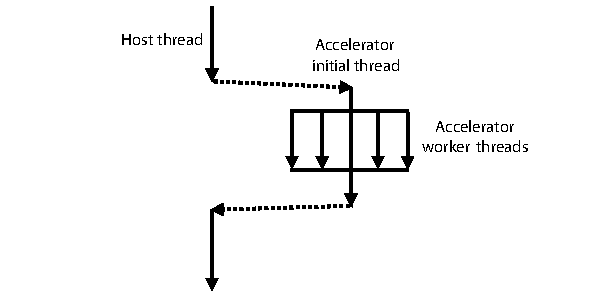
\includegraphics[clip=true,scale=1.00]
         {./06.heterogeneous_systems/figures/chapter-6-device-exec-model.pdf}
     }
\caption{ \textbf{The heterogeneous programming model supported by OpenMP} -- \small
        Program execution begins on the host device.  When a host device
        thread encounters a \texttt{target} construct, a new initial thread 
        executes the target region.  When the initial thread encounters
        a \texttt{parallel} construct it becomes the master of a
        teams of threads.
        }
\label{figure:chapter-6-device-exec-model}
\end{figure*}

After \OMPfourzero\ and the addition of the \code{target} construct, multiple
initial threads could arise during the execution of a program.  A
\emph{target}~\emph{region} is all of the code that is dynamically encountered
during the execution of a \code{target} construct.  As shown in
Figure~\ref{figure:chapter-6-device-exec-model}, the thread that encounters a
\code{target} construct does not itself execute the target region.  Instead, a
new initial thread begins the execution of the target region.  Each
target region acts as an \OMP\ sub-program where an initial thread begins the
execution of the sub-program.  The initial thread may encounter
other parallel constructs and spawn teams of threads. 

The initial thread that executes a target region is potentially running on an
accelerator.  We say potentially because it's possible that the OpenMP
program is running on a system that has no accelerators, in which case, the
target region is executed by an initial thread running on the host device.
Even on systems where accelerators are available, if the \code{target}
construct has an \code{if} clause whose conditional expression evaluates to
\emph{false} then the initial thread executes on the host device (see
Section~\ref{ssec:06.if-clause}).  If there are multiple accelerators
available, the \code{device} clause %(see Section~\ref{ssec:06.device-clause})
can be used to select one of them.  When a \code{device} clause is not present,
the initial thread executes on the default device specified by the
\emph{default-device-var} ICV.
% Ruud - Changed to a "D" for consistency.
\index{Accelerators!Default-device-var ICV}
\index{ICV!default-device-var}

By default, the thread that encounters the \code{target} construct waits for
the execution of the target region to complete and then continues executing the
code after the \code{target} construct.  Note how this is different from a
\code{parallel} construct where the thread that encounters the construct
becomes the master thread in a team of threads that is created to execute the
parallel region.  

%-----------------------------------------------------------------------
%------------------------- New subsection ------------------------------
%-----------------------------------------------------------------------
\subsection{Contention Groups}
\label{ssec:06.contention-groups}
\index{Accelerators!Contention group}
\index{Accelerators!Initial thread}
\index{Contention group}

A \emph{contention group} is the set of all threads that are descendants of an
initial thread.  An initial thread is never a descendant of another initial
thread.  Each dynamically encountered \code{target} construct starts a new
contention group.  

Threads in different contention groups cannot synchronize with
each other.  This means that threads that arise from different target regions
cannot synchronize with each other.  Further, the threads in the contention
group formed by the initial thread that started the execution of the program
cannot synchronize with any threads that arise from target regions.  This
restriction effectively limits how threads in contention groups (often threads
on different devices) can interact with each other.

When threads from different contention groups execute in parallel, only
variables\footnote{The size of these variables must be less than or equal 64 bits.} 
written to atomically 
(using an \code{atomic} construct)
by a thread in one contention group can be read by a thread in another contention group, and only
if both contention groups are executing on the same device.

%-----------------------------------------------------------------------
%------------------------- New subsection ------------------------------
%-----------------------------------------------------------------------
\subsection{A League of Teams}
\label{ssec:06.league-of-teams}
\index{Accelerators!League}
\index{Accelerators!Contention group}
\index{Accelerators!Initial thread}
\index{Contention group}

The \code{target}~\code{teams} construct %(see Section~\ref{sec:06.teams-construct}) 
starts a \emph{league} of teams executing
on an accelerator. Each of these teams is a single initial thread executing
in parallel the subsequent code statement.  This is similar to a
\code{parallel} construct but different in that each thread is its own team: a
team of one.  Threads in different teams are in different contention groups
and, therefore, restricted in how they can synchronize with each other.  

When a \code{parallel} construct is encountered by a league, each initial
thread in the league becomes the master of a new team of threads. The result is
a league of teams where each team has one or more threads. Each team is a
contention group.  Each team of threads then concurrently executes the parallel
region.

Leagues are used to express a type of loosely connected parallelism where teams
of threads execute in parallel but with very limited interaction across teams.
We will explore this more later in Section~\ref{ssec:06.distribute-construct}
when we discuss how leagues are used in accelerated worksharing.

%-----------------------------------------------------------------------
%------------------------- New subsection ------------------------------
%-----------------------------------------------------------------------
\subsection{The Target Task}
\label{ssec:06.target-task}
\index{Tasking!Creation}
\index{Creation of tasks}
\index{Accelerators!Target task}

Sometimes we don't want the host thread that encounters a target region to wait
for the target region to complete.  We want the target region to execute
asynchronously so that the host thread can go off and do other work.
\OMP\ already has tasks that provide capabilities for launching and
coordinating the asynchronous execution of code regions.  Leveraging these
features, the device constructs are formulated as \OMP\ task generating
constructs. 
\index{Accelerators!Device constructs}

We have been talking in terms of threads up to this point, but recall that
threads are the entities that do work; the actual work is a task.  There is
always a task (implicit or explicit) that a thread is executing.  Tasks are
executed only by threads running on the device where the tasks were generated.

The \code{target} construct is a task-generating construct.  When a thread
encounters a \code{target} construct, it generates an explicit task that
manages the execution of the target region.  The \OMPfourfive\ specification
refers to this task as the \emph{target task}.  This is an unfortunate name as
it seems to imply that the target task is running on an accelerator, but it
is an explicit task generated on the host.  The target task is complete when
the enclosed target region is complete.

\index{Accelerators!Initial thread}
When the target task executes, the target region executes in the context of an
implicit task, called an \emph{initial task}, on the accelerator.  The initial
task is executed by the initial thread.  Before \OMPfourzero\, there was only one
initial task; the implicit task that enclosed the whole program.  However, now each
time a target region executes, a new initial task is generated on the target
device.  The target task is complete when the initial task, and thus the target
region, is complete.

\index{Accelerators!Generating task}
The task that the host thread is executing when it encounters the \code{target}
construct is called the \emph{generating task}.  It generates the target task.
Because the \code{target} construct results in a task, we now have available
all of the asynchronous execution features from \OMP\ tasking.

\begin{figure*}[!tb]
\centering
\pdfimageresolution 400
\fbox{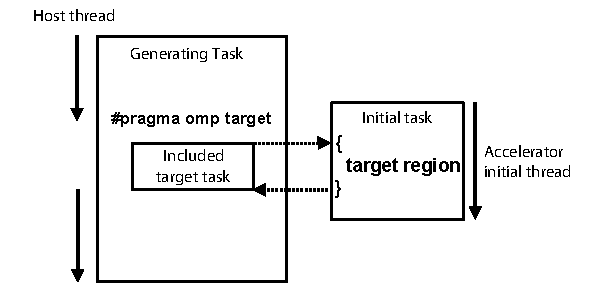
\includegraphics[clip=true,scale=1.00]
         {./06.heterogeneous_systems/figures/chapter-6-device-task-model1.pdf}
     }
\caption{ \textbf{The target task as an included task} -- \small
        By default, the target task is an included task.  The
        generating task cannot resume until the included target
        task is complete.  The target task completes when the
        implicit task that contains the target region is completed
        by the initial thread running on an accelerator.
        }
\label{figure:chapter-6-device-task-model1}
\end{figure*}

\index{Tasking!Included task}
\index{Accelerators!Included task}
\index{Included task}
As shown in Figure~\ref{figure:chapter-6-device-task-model1}, the target
task is executed immediately by the thread that is executing the generating
task.  The thread suspends executing the generating task and begins executing
the target task.  The target task is by default an \emph{included task}.  It is
a feature of the \OMP\ tasking model that the task that generates an included
task cannot be scheduled to execute until the included task is complete.  For
our purposes, the effect is that execution cannot continue after a
\code{target} construct until the target region is complete.

\begin{figure*}[!tb]
\centering
\pdfimageresolution 400
\fbox{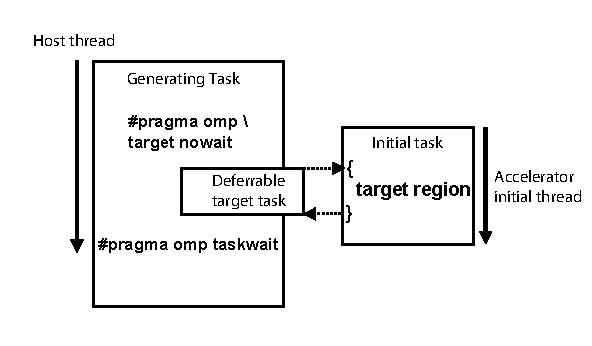
\includegraphics[clip=true,scale=1.00]
         {./06.heterogeneous_systems/figures/chapter-6-device-task-model2.pdf}
     }
\caption{ \textbf{The target task as a deferrable task} -- \small
        The nowait clause makes the target task a deferrable task.  The
        generating task may now be scheduled to execute before the target
        task is complete.  The effect is that the generating task may
        execute in parallel with the target task.
        }
\label{figure:chapter-6-device-task-model2}
\end{figure*}

However, sometimes we want the host device to do useful work in parallel with
the accelerator device. Figure~\ref{figure:chapter-6-device-task-model2} shows
how the \code{nowait} clause solves this problem.  The \code{nowait} clause
changes the default behavior of the target task so that it is no longer an
included task %(see Section~\ref{sec:06.async-exec}).  
With a \code{nowait}
clause, the target task is like any other deferrable task.  

Once a thread suspends execution of a target task, it is available to execute
other tasks, including the original task that generated the target task.  The
effect is that execution of the generating task may continue past the
\code{target} construct and before the associated target region has completed.
The generating task is not stuck waiting for the target task (and thus the
target region) to complete.  The \OMP\ task synchronization features,
introduced in Chapter~\ref{chap:tasking}, may be used to determine
when the target task is complete.

For example, in Figure~\ref{figure:chapter6-nowait} the thread that encounters the
\code{target} construct generates a task and then continues after the
construct to execute the function \code{F()}.  The target task
and the function \code{F()} are potentially executed in parallel.  The host
thread then waits at the \code{taskwait} construct to ensure that the target
task has completed.

\begin{figure*}[!tbh]
\begin{verbatim}
 1 #pragma omp target map(a,b,c,d) nowait // Generate target task
 2 {
 3   #pragma parallel for
 4   for (i=0; i<N; i++) {
 5     a[i] =  b[i] * c + d;
 6   }
 7 } // End of target
 8 
 9 F(b); // Execute in parallel with target task
10
11 #pragma omp taskwait // Wait for target task to finish
\end{verbatim}
\caption{ \textbf {Code fragment with a target nowait region} -- \small
          The encountering thread generates a target task 
          and then continues past the target construct
          to execute the function \emph{F()}.
         }
\label{figure:chapter6-nowait}
\end{figure*}

%In Section~\ref{sec:06.async-exec} we will show more asynchronous execution
%examples using the \code{nowait} clause along with the \code{taskwait}
%construct and \code{depend} clause to demonstrate how to coordinate the
%asynchronous execution of target regions by leveraging the power of \OMP\
%tasks.

%-----------------------------------------------------------------------
%------------------------- New section ---------------------------------
%-----------------------------------------------------------------------
\section{Heterogeneous Memory Model}
\label{ssec:06.heterogeneous-memory-model}

\index{Accelerators!Device constructs}
%Code executing on a device is typically not very useful without some data to
%compute on.  
This section provides an overview of the \OMP\ heterogeneous memory model.
The device constructs, clauses, and runtime functions that control how data is shared
between threads executing on the host and an accelerator device are listed below:

\begin{itemize}
  \item Map and Defaultmap Clauses
  \item Target Data Construct
  \item Target Enter and Exit Data Constructs
  \item Target Update Construct
  \item Declare Target Directive
  \item Use\_device\_ptr and Is\_device\_ptr Clauses
  \item Device Memory Functions
%  \item Runtime Functions
%  \begin{itemize}
%    \item \code{omp_target_alloc}
%    \item \code{omp_target_free}
%    \item \code{omp_target_is_present}
%    \item \code{omp_target_memcpy}
%    \item \code{omp_target_memcpy_rect}
%    \item \code{omp_target_associate_ptr}
%    \item \code{omp_target_disassociate_ptr} 
%  \end{itemize}
\end{itemize}

\index{OpenMP clauses!map}
\index{Accelerators!Map clause}
Of these, by far the most important is the \code{map} clause.  Recall from
Chapter~\ref{chap:recap} that variables are shared or private.  As of \OMPfourzero,
variables can also be \emph{mapped}, which is the concept that \OMP\ uses to
describe how data is shared across devices.  The \code{defaultmap} clause can
change the default rules for determining if certain variables are either
private or mapped.  The general concepts of mapped variables
are discussed later in this section.  
The syntax and mechanics of the \code{map} and \code{defaultmap} clauses
are covered in Section~\ref{sec:06.data-mapping-clauses}.

The host and accelerator may have different representations for the address of
a variable.  The \code{use_device_ptr} and \code{is_device_ptr} clauses are
provided for the instances in which this difference in address representation
must be dealt with explicitly.  These device pointer clauses are covered in
Section~\ref{sec:06.Device-pointer-clauses}.

Variable's with static storage (for example, global variables) may be mapped
for the entire program using the \code{declare target} directive, which is
covered in Section~\ref{sec:06.declare-target-construct}.

The \code{target}~\code{data}, \code{target}~\code{enter}~\code{data},
\code{target}~\code{exit}~\code{data}, and \code{target}~\code{update}
constructs are used to reduce the performance overhead of copying data between
the host and an accelerator.  These data-mapping constructs are
covered in Section~\ref{sec:06.data_mapping_constructs}.

The device memory functions are described in detail in
Section~\ref{ssec:02.new_runtime_functions_3} starting on
page~\pageref{ssec:02.new_runtime_functions_3}.  
The \code{omp_target_is_present} function determines if a variable
is mapped.  Otherwise, the other device memory functions 
manage dynamically allocated device memory.  
Section~\ref{sec:06.device-memory-routines} has examples 
that demonstrate how to use these functions.
%These low-level functions are
%essential for more advanced operations.

%-----------------------------------------------------------------------
%------------------------- New subsection ------------------------------
%-----------------------------------------------------------------------
\subsection{Mapped Variables}
\label{ssec:06.mapped-variables}
\index{Mapped variable}

\index{Accelerators!Initial thread}
Threads executing on an accelerator can have private variables.  The initial
thread that begins the execution of a target region gets a private instance of
a variable that appears in a \code{private} or \code{firstprivate} clause on the
\code{target} construct.  For a \code{firstprivate} clause, the private variable
is initialized with the value of the original variable from the host thread
that encountered the construct.  Likewise, any automatic (stack)
variables that are declared in a scope contained within the construct
are private to the initial thread.

%How do the host and accelerator threads share variables?  
\OMP\ threads 
share variables that are stored in a single shared memory.  However, 
heterogeneous architectures do not always have memory that is symmetrically shared between
host and accelerator devices.  A very common example of a 
heterogeneous architecture like this is one where the accelerator is a card 
and communication to the accelerator occurs over a PCIE bus. 

As shown in figure~\ref{figure:chapter-6-device-memory-types}, \OMP\ supports
heterogeneous architectures with both distributed and shared memory by \emph{mapping}
variables from the host to an accelerator.
When the host and accelerator device do not share memory, a mapped variable
is copied from the host's memory into the accelerator's local memory.
Mapping hides whether or not a variable is shared by or copied to a device.
Based on a heterogeneous architecture's memory system, the \OMP\
implementation does what is required, either sharing or copying a variable when it
is mapped.

\begin{figure*}[!tbhp]
\centering
\pdfimageresolution 400
\fbox{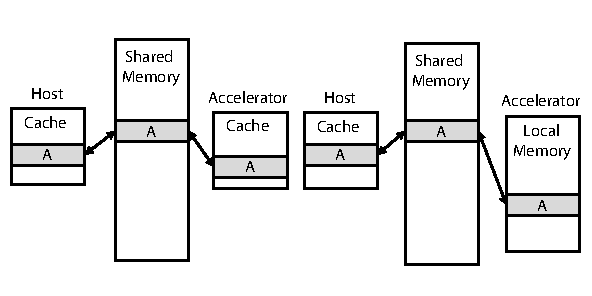
\includegraphics[clip=true,scale=1.00]
         {./06.heterogeneous_systems/figures/chapter-6-device-memory-types.pdf}
     }
\caption{ \textbf{A mapped variable in shared or distributed memory} -- \small
        A mapped variable may be in either shared or distributed memory.
        The OpenMP implementation determines if copies are required.
        }
\label{figure:chapter-6-device-memory-types}
\end{figure*}

\index{Memory consistency!Model} 
How does one ensure that threads on different devices see the same
value of a mapped variable and when?  For the most part, the \OMP\ memory
consistency model as outlined in Chapter~\ref{ssec:01.memory_model}, starting on
page~\pageref{ssec:01.memory_model}, is extended to mapped variables.  

A mapped variable is similar to a shared variable.  Without some 
type of synchronization, two threads executing on
different devices cannot simultaneously access the same mapped variable if
either of the threads writes to the variable.  

\index{OpenMP clauses!map}
\index{Accelerators!Map clause}
Threads executing on different devices may see a consistent value of a mapped
variable at points that are determined by the effects of the \code{map} clause
and the \code{target update} construct.

If memory is distributed, then mapping a variable requires memory allocation,
copy, and flush operations.  The allocation and copy operations are not
required (or are trivial) when memory is shared, but the flush
operation is still necessary.  Although the underlying machinations of variable mapping
is handled by the \OMP\ implementation, it is important to be aware
of the dual-nature of mapped variables to write programs that 
achieve good performance across different architectures.  

%Because the instances of a mapped variable may be in different address spaces,
Because two devices may not share the same address space,
the address of a mapped variable may not be the same on two devices
When a pointer variable is mapped, only the pointer is synchronized, not the
block of memory it points to.  However, array sections may be used to map the
pointed-to memory.

%\index{OpenMP clauses!map}
%\index{Accelerators!Map clause}
%Variables are explicitly mapped using the \code{map} clause (see
%Section~\ref{sec:06.map-clause}).  For variables referenced in a \code{target}
%construct that do not appear in a \code{map}, \code{private},
%\code{firstprivate} or \code{is_device_ptr} clause, data-mapping rules
%determine if they are mapped or private (see
%Section~\ref{ssec:06.defaultmap-clause}).

%Since there might be two copies of the variable, there is a policy for
%maintaining the consistency of the different copies of the variable.
%For example, if a thread on the accelerator writes to a mapped variable, when
%can a thread on the host device see the updated value of the variable?  

%-----------------------------------------------------------------------
%------------------------- New subsection ------------------------------
%-----------------------------------------------------------------------
\subsection{Device Data Environments}
\label{ssec:06.device-data-environments}

\index{Accelerators!Device data environment}
\index{Device data environment}
An accelerator has a \emph{device data environment} that contains the set of
all variables currently accessible by threads running on that device.  As we
discussed in the previous section, host threads share variables with target
device threads by mapping them.  Mapping a variable ensures that the variable
is in the data environment of an accelerator.

\index{Device data environment!Orginal variable}
\index{Device data environment!Corresponding variable}
An \emph{original} variable in a host thread's data environment is mapped to a
\emph{corresponding} variable in the accelerator's data environment.
Depending on the availability of shared memory between the host and target
devices, the original and corresponding variables are either the same variable
allocated in shared memory, or they are allocated in different memories and
copy operations are required to keep the original and corresponding variables
consistent. Whether a mapped variable uses shared or distributed memory is 
taken care of by the \OMP\ implementation.

\index{Device data environment!Present in}
There only can be one instance of a variable in a device data environment.  The
\OMP\ implementation keeps track of which variables are mapped.  If a variable
is already \emph{present} in a device data environment, mapping it again will
find the variable is already there and increment a reference count.  It
will not allocate another instance of the variable.

Minimizing the transfer of data between the host and an accelerator is often
critical to getting good performance on heterogeneous architectures.
Repetitively mapping a variable that is reused by multiple \code{target}
constructs is potentially inefficient.  The \code{target}~\code{data},
\code{target enter data} and \code{target}~\code{exit}~\code{data} constructs amortize data
transfers by mapping variables across the execution of multiple \code{target}
constructs.  Further, the \code{declare}~\code{target} construct can map static and
global variables for the whole program.  Once a variable is mapped to an
accelerator, situations can arise where the value of the variable must be
updated from or to the device, and the \code{target}~\code{update}
construct fulfills this need.  The \code{omp_target_is_present} runtime
function is used to test if a variable is mapped.  
\index{Accelerators!omp\_target\_is\_present} 
\index{OpenMP runtime functions!omp\_target\_is\_present} 

%-----------------------------------------------------------------------
%------------------------- New subsection ------------------------------
%-----------------------------------------------------------------------
\subsection{Device Pointers}
\label{ssec:06.device-pointers}

\index{Accelerators!Device constructs}
Because shared and distributed memory is supported, the \OMP\ memory model
assumes that the host and accelerator data environments are in different
address spaces.  However, this assumption creates some restrictions on
accessing the address of the variable.
% Ruud - I hope this change is OK
% A programmer using the \OMP\ device constructs must be aware of the different
With the \OMP\ device constructs, the user must be aware of the different
address spaces and be careful when using pointers.  
If the host and accelerator do not share memory, their local memories are in
different address spaces.  When a variable is mapped to an accelerator's data
environment, a copy occurs, and the address of the variable on the accelerator
is not the same as the address of the variable on the host.

Memory addresses are stored in pointer variables.  A host thread cannot access
memory via a pointer variable that contains an accelerator address.  Likewise,
an accelerator thread cannot access memory via a pointer variable that contains
a host address.  
Further, the host and accelerator may have different representations for the
address of a variable.  For example, the value of a memory address might
require 64 bits on a host and 32 bits on an accelerator.

In Figure~\ref{figure:chapter6-devptr1}, the host pointer variable \code{hptr} is
assigned the address of a memory location in the host's address space.  
Mapping \code{hptr} copies the value of the pointer variable to the accelerator. The
access to \code{hptr} at line $6$ in the target region by an accelerator thread is illegal.
The accelerator thread is attempting to access a host address.

Likewise in Figure~\ref{figure:chapter6-devptr2}, the accelerator pointer
variable \code{dptr} is assigned the address of a memory location in the
accelerator's address space.  The access to \code{dptr} at line $7$ by a host thread is illegal.

\begin{figure*}[!tb]
\begin{verbatim}
1   char *hptr = malloc(N);
2
3   // Error - Accessing a host address on accelerator
4   #pragma omp target map(hptr)
5   for (int i=0; i<N; i++)
6     *hptr++ = 0;
\end{verbatim}
\caption{ \textbf {Illegal access of a host memory address } -- \small
          A pointer variable containing a host memory address cannot be
          de-referenced by an accelerator thread.
         }
\label{figure:chapter6-devptr1}
\end{figure*}

\begin{figure*}[!tb]
\begin{verbatim}
1   char *dptr;
2   #pragma omp target map(dptr)
3   dptr = malloc(N);
4
5   // Error - Accessing a device address on host
6   for (int i=0; i<N; i++)
7     *dptr++ = 0;
\end{verbatim}
\caption{ \textbf {Illegal access of an accelerator memory address} -- \small
          A pointer variable containing an accelerator memory address 
          cannot be de-referenced by a host thread.
         }
\label{figure:chapter6-devptr2}
\end{figure*}

\index{Accelerators!Device data environment}
\index{Device data environment}
\index{Accelerators!Device pointer}
\index{Device pointer}
A \emph{device pointer} \index{Accelerators!Device pointer} is a pointer
variable in the host data environment whose value is an object that contains
the address of a storage location in an accelerator's device data environment.  

Note that the value of a device pointer is an object.  How the
value of a device address is represented on a host is not necessarily the same
way that it is represented on an accelerator.  
When a device pointer is referenced in a target construct, the compiler
may need to transform the representation of the device address stored in
the device pointer.

%If a device pointer is stored in
%a host pointer, then the compiler needs to transform the representation of that
%pointer when it is used on the device.  

%The \code{use_device_ptr} and \code{is_device_ptr} 
%clauses are provided for the instances in which the difference in address
%representation between the host and accelerator must be dealt with explicitly.
%\index{Accelerators!Is\_device\_ptr clause}
%\index{OpenMP clauses!is\_device\_ptr}
%\index{Accelerators!Use\_device\_ptr clause}
%\index{OpenMP clauses!use\_device\_ptr}
%We need to indicate that a variable is a device pointer when it is referenced
%in a \code{target} construct.  

%The \code{omp_target_alloc} 
%function, described in detail in Section~\ref{ssec:02.new_runtime_functions_3},
%allocates storage in an accelerator's
%device data environment and returns a device pointer.  The function cannot be
%called inside a target region.  

\index{OpenMP clauses!is\_device\_ptr}
\index{Accelerators!Is\_device\_ptr clause}
In Figure~\ref{figure:chapter6-devptr3}, the \code{omp_target_alloc} function
returns a device address.  The device pointer \code{dptr} must appear in an
\code{is_device_ptr} clause on the \code{target} construct to correctly refer
to it in the target region.  The variable \code{dptr} is private in the target
region.  On entry to the region, the private \code{dptr} variable is initialized
with the accelerator's memory address that corresponds to the original value of
\code{dptr} before the region (the host's representation of the device address).
See Section~\ref{sec:06.Device-pointer-clauses} for more details on device
pointers.

\begin{figure*}[!tb]
\begin{verbatim}
1   int dev = omp_get_default_device();
2   char *dptr = omp_target_alloc(dev, n);
3 
4   #pragma omp target is_device_ptr(dptr)
5   for (int i=0; i<n; i++)
6     *dptr++ = 0;
\end{verbatim}
\caption{ \textbf {Legal access of an accelerator memory address using a device pointer} -- \small
          A device pointer variable that appears in an \texttt{is\_device\_ptr} clause 
          may be de-referenced in a target region.
        }
\label{figure:chapter6-devptr3}
\end{figure*}


%-----------------------------------------------------------------------
%------------------------- New subsection ------------------------------
%-----------------------------------------------------------------------
\subsection{Array Sections}
\label{ssec:06.array-sections}
\index{Array section}
\index{Mapped variable!Array section}

Pointer variables are used extensively in C and C++.  The value stored in a
pointer variable is the address of another variable.  As we saw in the last
section, in order to support a variety of systems, the \OMP\ model assumes that
the host and accelerator may not share the same address space. Thus, mapping a
pointer variable by itself is not very useful.  We want to map the pointed-to
variable (the memory that the pointer references). In order to map the
pointed-to variable, we need to know its size.

For C and C++, we need something in the \OMP\ syntax to express the concept of
mapping the pointed-to variables.  This is one of the reasons that \OMPfourzero\
added \emph{array}~\emph{section} syntax for array and pointer 
variables.\footnote{Array sections may also appear in the \code{depend} clause.}

An array section is a subset of the elements in an array.  In \OMP\, array
sections are restricted to a contiguous set of elements.  The C and C++ array
subscript syntax is extended to support an array section expression.  The
array section syntax \code{base[\emph{offset}:\emph{length}]} is described below:

\begin{itemize}

  \item The $base$ is a C or C++ variable name with array, pointer type, or
  in C++, reference to array or reference to pointer type.

  \item The $offset$ is an non-negative integer expression that is an offset
  from the start of the array.  The $offset$ is optional and, if not specified,
  defaults to 0.

  \item The $length$ is a non-negative integer expression that is the length
  of the array section.   If the $base$ variable has a type of array or
  reference to array, then the $length$ is optional and defaults to the
  number of elements in the array.  If the $base$ variable has a type of
  pointer or reference to pointer, then the $length$ must be specified.

%  \item The $stride$ is a (non-negative) integer expression that, when it is
%  greater than one, selects non-contiguous elements from the array.  The
%  $stride$ is optional and defaults to one.  
%  
\end{itemize}

\index{Array section!Pointer-based}
The value of a pointer variable used in an array section is the address of a
pointed-to array variable.  The pointed-to array variable may or may not have
been dynamically allocated.  Even if the pointed-to variable is a single scalar
variable, when it's used in an array section, it is an array of one element.

An array section is \emph{pointer-based} when the $base$ is a pointer variable.
A pointer-based array section is mapped using the following steps: \begin{enumerate}

  \item Create a pointer variable in the accelerator's data environment.

  \item Map the host's pointed-to variable to the accelerator's data
  environment.

  \item Initialize the accelerator's pointer variable with the address of the
  pointed-to variable in the accelerator's address space.

\end{enumerate}

In Figure~\ref{figure:chapter6-array-sections1}, the host pointer variable
\code{hptr} is assigned the address of a storage location in the host's data
environment.  The array section \code{hptr[0:1024]} is then mapped to the
accelerator's data environment.  The 1024 element array pointed to by \code{hptr} is
mapped to the accelerator.  The \code{hptr} pointer variable is not mapped but is
private in the target region and initialized with the address of the pointed-to
array. Compare this to Figure~\ref{figure:chapter6-devptr1}.

\begin{figure*}[!tbhp]
\begin{verbatim}
1   char *hptr;
2
3   hptr = malloc(1024);
4
5   // Map an array section.
6   #pragma omp target map(hptr[0:1024])
7   for (int i=0; i<N; i++)
8     hptr[i] = 0;
9   
\end{verbatim}
\caption{ \textbf {Map a pointer-based array section} -- \small
          Use an array section to map pointed-to memory.
         }
\label{figure:chapter6-array-sections1}
\end{figure*}

\index{Array section!Examples}
\index{OpenMP clauses!map}
\index{Accelerators!Map clause}
Array sections are available in the Fortran base language.  In C/C++, an
array section may appear only as a list item in an \OMP\ \code{map} or
\code{depend} clause.  The C/C++ base language was not extended to support
array sections.  Some examples of array sections in C/C++ are shown
in Figure~\ref{figure:chapter6-map-ptr1}

\begin{figure*}[!tbhp]
\begin{verbatim}
 1 float *p = malloc(N);
 2 float a[N];
 3
 4 // Map pointer based array section
 5 map(p[0:N:1]) 
 6 map(p[0:N])
 7 map(p[:N])
 8
 9 // Map array based array section
10 map(A[0:N:1])
11 map(A[0:N])
12 map(A[:N])
13 map(A[:]) // Size is N
14 
15 // Map array section with offset
16 map(p[32:N-32]
17 map(A[N/2:N/4]
18
\end{verbatim}
\caption{ \textbf {Array section syntax examples} -- \small
          Various usage of array section syntax in C and C++.
         }
\label{figure:chapter6-map-ptr1}
\end{figure*}

\index{Array section!Array slice}
Array sections are also useful for mapping a slice of an array.  It might be
that mapping a very large array exceeds the storage capacity of the
accelerator's local memory.  In this case, we would like to map slices of the
array and then compute on each slice.  Figure~\ref{figure:chapter6-mapslice}
shows how this can be done.

\begin{figure*}[!tb]
\begin{verbatim}
 1 #define BIG 256
 2 #define N (1024*1024)
 3 int a[N*BIG];
 4 
 5 void F(const int c, const int d)
 6 {
 7   for (int k=0; k<N*BIG; k+=N) {
 8     #pragma omp target map(from:a[k:N]) firstprivate(c,d) 
 9     for (int i=0; i<N; i++) {
10       a[k+i] =  k+i * (c + d);
11     } // End of target
12   }
13 }
\end{verbatim}
\caption{ \textbf {Use array section to map a subset of an array} -- \small
          Map a slice of the array \texttt{a} each time through the loop.
         }
\label{figure:chapter6-mapslice}
\end{figure*}

The rest of the sections in this chapter describe 
the syntax and semantics of the device constructs and clauses.

%-----------------------------------------------------------------------
%------------------------- New section ---------------------------------
%-----------------------------------------------------------------------
\section{The Target Construct}
\label{sec:06.target-construct}
\index{OpenMP constructs!Target}
\index{Accelerators!Target}

\index{Accelerators!Initial thread}
The purpose of the \code{target} construct is to offload the execution of code
to an accelerator.  The code in a target region is executed by a new
initial thread.  
The code in Figure~\ref{figure:chapter6-hello} is a simple 
hello world example that uses the \code{target} construct.  

\begin{figure*}[!tbhp]
\begin{verbatim}
 1 #include <stdio.h>
 2 #include <omp.h>
 3 void hello(void)
 4 {
 5   #pragma omp target 
 6   {
 7     if (!omp_is_initial_device())
 8       printf("Hello World from accelerator\n");
 9     else
10       printf("Hello World from host\n");
11   }
12 }
\end{verbatim}
\caption{ \textbf {Example of a target construct } -- \small
          If the initial thread is running on an accelerator, it executes the
          first \texttt{printf()}.
          Otherwise, it is running on the host device and
          executes the second \texttt{printf()}.
          Note that some implementations may not support calling \texttt{printf()} on an accelerator. 
         }
\label{figure:chapter6-hello}
\end{figure*}

\index{Accelerators!omp\_is\_initial\_device}
\index{OpenMP runtime functions!omp\_is\_initial\_device}
The \OMP\ runtime function
\code{omp_is_initial_device} returns true if the code is executing on the
host device.  If there are no accelerators on the system where the code is
running, then the initial thread that executes the target region runs on the host
device.  

\index{Accelerators!Device constructs}
\index{Accelerators!Host fall back} 
Since the initial thread that executes the target region can always 
\emph{fall back} to the host, programs that use device constructs are
portable to systems that do not have accelerators. However, in the following
description of the \code{target} construct it is assumed that the code is
running on a system with at least one accelerator.  

The \code{target} construct syntax in C/C++ and Fortran is given in
Figure~\ref{figure:syntax-target-construct}.  The clauses that are available on
the \code{target} construct are listed in
Figure~\ref{figure:syntax-target-clauses}.

\begin{figure}[!htbp]
\centering
\begin{tabular}{|l|}
\hline
\ompbctarget \ompclauses  \\
\hspace{2em}\emph{structured block} \\
\hline

\ompbftarget \ompclauses \\
\hspace{2em}\emph{structured block} \\
\ompbftargetend \\
\hline

\end{tabular}
\caption{ \textbf{Syntax of the target construct in C/C++ and Fortran} -- \small
          A target region is executed by an
          initial thread running on an accelerator.
          }
\label{figure:syntax-target-construct}
\end{figure}

\index{OpenMP clauses!if}
\index{OpenMP clauses!map}
\index{OpenMP clauses!device}
\index{OpenMP clauses!private}
\index{OpenMP clauses!firstprivate}
\index{OpenMP clauses!is\_device\_ptr}
\index{OpenMP clauses!defaultmap}
\index{OpenMP clauses!nowait}
\index{OpenMP clauses!depend}
\index{Accelerators!If clause}
\index{Accelerators!Map clause}
\index{Accelerators!Device clause}
\index{Accelerators!Private clause}
\index{Accelerators!Firstprivate clause}
\index{Accelerators!Is\_device\_ptr clause}
\index{Accelerators!Defaultmap clause}
\index{Accelerators!Nowait clause}
\index{Accelerators!Depend clause}
\begin{figure}[!htbp]
\centering
\begin{tabular}{|l l|}
\hline
\bciftarget & (C/C++)\\
\bfiftarget & (Fortran)\\
\bmap & \\
\bcdevice & (C/C++)\\
\bfdevice & (Fortran)\\
\bprivate & \\
\bfirstprivate & \\
\bisdeviceptr & \\
\bdefaultmap & \\
\bnowait & \\
\bdepend & \\
\hline

\end{tabular}
\caption{ \textbf{Clauses supported by the target construct} -- \small
          The \texttt{if} and \texttt{device} clauses are discussed in
          Section~\ref{sec:06.which-device}. The \texttt{map} clause is discussed in
          Section~\ref{sec:06.map-clause}.  The \texttt{nowait} and \texttt{depend} clauses are
          discussed in Section~\ref{sec:06.async-exec}.  The \texttt{is\_device\_ptr}
          clause is discussed in Section~\ref{ssec:06.device-pointers} The
          \texttt{defaultmap} clause is discussed in 
          Section~\ref{ssec:06.defaultmap-clause}.
          }
\label{figure:syntax-target-clauses}
\end{figure}

\index{Accelerators!Target task}
The \code{target} construct is a task generating construct.  When a thread
encounters a \code{target} construct a target task is generated on the host
device.  You can think of the target task as a task bound to the host
device that wraps the exection of the target region.  The target task is
complete (on the host) when the target region is complete (on the accelerator).
The \code{nowait} and \code{depend} clauses affect the type and asynchronous
behavior of the target task. 

By default, the execution of the target task is synchronous.  The encountering
thread cannot continue past the target construct until the target task is
complete.  The \code{nowait} clause makes the execution of the target region
asynchronous.  After generating the target task, the encountering thread does
not wait for the target task to complete, but instead it can continue and
execute the code after the \code{target} construct.  Task scheduling via
the \code{taskwait} cosntruct or the \code{depend} clause may be used to
synchronize with the completion of the target task.  The execution model of the
\code{target} construct is covered in detail in
Section~\ref{sec:06.execution-model}.

% Ruud - Changed to a "D" for consistency.
\index{Accelerators!Default-device-var ICV}
\index{ICV!default-device-var}
\index{Accelerators!Host fall back} 
The target region is executed by an initial thread.  Where the initial thread
runs (the host or an accelerator) is determined by the \emph{default-device-var}
ICV. The \code{device} clause can be used to specify a device other than the
default.  The \code{if} clause is available to conditionally fall back to
running the initial thread on the host.

The initial thread gets a private instance of a variable that appears in a
\code{private} or \code{firstprivate} clause on a \code{target} construct.  For
a \code{firstprivate} clause, the private variable is initialized with the value
of the original variable from the host thread that encountered the target
construct.  Likewise, any automatic (stack) variables that are declared in a
scope contained within the target construct are private to the initial thread.

Variables that appear in \code{map} clauses are mapped.  Any assignments 
specified by a \code{map} clause occur when the target task executes. 
If a variable referenced in the \code{target} construct does not appear in a
\code{map}, \code{private}, \code{firstprivate} or \code{is_device_ptr} clause,
then default data-mapping rules determine if and how the variable is mapped
(see Section~\ref{sec:06.data-mapping-clauses}).

\index{Array section!Pointer-based}
C/C++ pointer variables that appear in \code{map} clauses as the base of an
array section are private in the target region. The private variables are 
initialized with the value
of the address of the array section's pointed-to memory in the accelerator's
address space.

The code in Figure~\ref{figure:chapter6-target-mxv} illustrates how to
use the \code{target} construct to offload to an accelerator the matrix times
vector product example taken from \cite{ChapmanEtAl:2007}.  By adding
the \code{target} construct at line $6$, the loop body is offloaded to an
accelerator.

\begin{figure*}[!tb]
\begin{verbatim}
 1 void mxv(int m, int n, double * restrict a,
 2          double * restrict b, double * restrict c)
 3 {
 4 
 5   #pragma omp target map(a[:n],b[:n],c[:n]) firstprivate(m,n)
 6   {
 7     int i, j;
 8     #pragma omp parallel for default(none) \
 9             shared(m,n,a,b,c) private(i,j)
10     for (i=0; i<m; i++)
11     {
12       a[i] = b[i*n]*c[0];
13       for (j=1; j<n; j++)
14         a[i] += b[i*n+j]*c[j];
15     } // End of parallel for
16   } // End of target
17 }
\end{verbatim}
\caption{ \textbf {Example using the target construct to execute the matrix 
                   times vector on an accelerator} -- \small
          The host thread waits for the execution of the target region to
          finish before it continues after the construct.
         }
\label{figure:chapter6-target-mxv}
\end{figure*}

When a host thread encounters the \code{target} construct at line $5$, it generates an
included target task, suspends the current task, and starts executing the
target task.  Because the target task is included, the host thread must
wait for the target region, and thus the target task to complete, before
continuing to execute the statement after the target construct.
Scalar variables that do not appear in a \code{map} clause default to
firstprivate, but for clarity the variables \code{m} and \code{n} are listed 
explicitly in a clause.
Because the variables \code{a}, \code{b}, and \code{c} are pointers, array sections are
required in the \code{map} clause to describe the size of the pointed-to
memory.  The pointer variables themselves are private in the target region.  

The array sections' pointed-to memory is mapped to the accelerator's address
space.
If the host and accelerator do not share memory, storage is allocated in the
accelerator's local memory, and the array sections are copied from the host's
memory to the accelerator's local memory.
The private pointer variables are assigned the address of the array section's
pointed-to memory in the accelerator's address space.
Because the variables \code{i} and \code{j} are declared in a scope enclosed in the
target construct at line $7$, they are private.

The target region is executed by an initial thread running on the default
accelerator.  The initial thread encounters the \code{parallel for}
worksharing construct at lines $8-9$ and becomes the master of a new team of
threads that work together to execute the for-loop at line $10$.  
The variables \code{m}, \code{n}, \code{a}, \code{b}, and \code{c} which were private to the initial
thread are now shared among the threads in the team.  The variables \code{i} and
\code{j} are private to each thread in the team.

If the host and accelerator do not share memory, then when the target region is
complete, the array sections are copied back from the accelerator's local
memory to the host's memory.  The storage allocated in the accelerator's local
memory is then released.  After the target region is complete, the target task
completes and the host thread starts executing again at line $17$ after the
\code{target} construct.

The restrictions on the usage of the \code{target} construct are as follows:

\begin{itemize}

\item A \code{target} construct cannot be nested inside a target region.

\item A \code{target}~\code{data}, \code{target}~\code{update}, \code{target}~\code{enter}~\code{data}, or \code{target}~\code{exit}~\code{data} construct cannnot be nested in a target region.

\item \code{threadprivate} variables cannot be accessed in a target region.

\item In C++ a virtual member function cannot be invoked on an object that was
not constructed on the accelerator.  The object cannot be a mapped variable.

\item In Fortran, if an array section is derived from a variable that has a
\code{POINTER} or \code{ALLOCATABLE} attribute, then the variable cannot be
modified in the target region.

\end{itemize}

%-----------------------------------------------------------------------
%------------------------- New section ---------------------------------
%-----------------------------------------------------------------------
\section{The Target Teams Construct}
\label{sec:06.teams-construct}
\index{OpenMP constructs!Target teams}
\index{Accelerators!Target teams}
\index{Accelerators!League}
\index{Accelerators!Initial thread}

Strictly speaking, \code{target teams} is a combined construct made up of the
\code{target} and \code{teams} constructs.  But since a
\code{teams} construct may appear only nested immediately inside a
\code{target} construct with no other intervening statements or declarations
between the two constructs, the two constructs are inseparable.
The \code{teams} construct syntax in C/C++ and Fortran is shown in
Figure~\ref{figure:syntax-teams-construct}.

\begin{figure}[!tb]
\centering
\begin{tabular}{|l|}
\hline
\ompbcteams \ompclauses  \\
\hspace{2em}\emph{structured block} \\
\hline
\ompbfteams \ompclauses \\
\hspace{2em}\emph{structured block} \\
\ompbfteamsend \\
\hline
\end{tabular}
\caption{ \textbf{Syntax of the teams construct in C/C++ and Fortran} -- \small
          Create a league of initial threads each in its own team.
          }
\label{figure:syntax-teams-construct}
\end{figure}

Similar to the \code{parallel} construct, the \code{target}~\code{teams} construct 
specifies that the subsequent code block should be run in parallel.
A \code{parallel} construct creates a team of threads, where the thread
that encountered the \code{parallel} construct becomes the master thread.  Each
thread in the team executes the parallel region.  
The \code{target}~\code{teams} construct starts a \emph{league} of initial
threads where each thread is in its own team.  Each initial thread executes the
teams region in parallel (see Section~\ref{ssec:06.contention-groups}).  One
can think of the \code{target} construct as a \code{target}~\code{teams}
construct that creates a league with only one initial thread.

%Work-sharing constructs, such
%as the loop construct, control how the threads in a team share the execution of
%code in the parallel region.
%As shown in Figure~\ref{figure:chapter6-teams-mxv}, 

\index{Accelerators!League}
When a \code{parallel}
construct is encountered by a league, each thread in the league becomes the
master of a new team of threads. The result is a league of teams where each
team has multiple threads.  Each team of threads concurrently executes the
parallel region.  

The clauses that may appear on
the \code{teams} construct are listed in Figure~\ref{figure:syntax-teams-clauses}.  
Clauses from both the \code{target}
and \code{teams} constructs may appear on the The \code{target}~\code{teams}
construct.  

\index{OpenMP clauses!num\_teams}
\index{OpenMP clauses!thread\_limit}
\index{OpenMP clauses!default}
\index{OpenMP clauses!private}
\index{OpenMP clauses!firstprivate}
\index{OpenMP clauses!shared}
\index{OpenMP clauses!reduction}
\index{Accelerators!Num\_teams clause}
\index{Accelerators!Thread\_limit clause}
\index{Accelerators!Default clause}
\index{Accelerators!Private clause}
\index{Accelerators!Firstprivate clause}
\index{Accelerators!Shared clause}
\index{Accelerators!Reduction clause}
\begin{figure}[!htbp]
\centering
\begin{tabular}{|l l|}
\hline
\bcnumteams & (C/C++)\\
\bfnumteams & (Fortran)\\
\bcthreadlimit & (C/C++)\\
\bfthreadlimit & (Fortran)\\
\bcdefault & (C/C++)\\
\bffdefault & (Fortran)\\
\bprivate & \\
\bfirstprivate & \\
\bshared & \\
\breduction & \\
\hline
\end{tabular}
\caption{ \textbf{Clauses supported by the teams construct} -- \small
          The \texttt{num\_teams} and \texttt{thread\_limits} clauses are 
          described below.
          }
\label{figure:syntax-teams-clauses}
\end{figure}

\index{Accelerators!Contention group}\index{Contention group}
The number of teams created by a \code{target}~\code{teams} construct is
implementation defined or is specified by the \code{num_teams} clause.  Each
team is executing in its own contention group.  The maximum number of threads
active in a contention group is specified by the \code{thread_limit} clause.  

What is the real difference between the \code{target}~\code{teams} and
\code{parallel} constructs? Both constructs fork multiple threads that execute
the subsequent block of code in parallel.  The \code{target teams} construct is
asserting a more restricted form of parallelism than the \code{parallel}
construct allows.  The compiler can take advantage of these restrictions and be
much more aggressive at exploiting parallelism.  These restrictions are as
follows:

\begin{itemize}

  \item Because the teams that are started by a \code{target teams}
  construct are each in their own contention group, threads from different 
  teams cannot synchronize with each other.

  \item The only \OMP\ constructs that can appear in a \code{teams} region
  are the \code{parallel}, \code{distribute} and any other \code{parallel} or
  \code{distribute} regions arising from related constructs.  These are
  listed here: \begin{itemize}
      \item \code{parallel} 
      \item \code{parallel for} (C/C++)
      \item \code{parallel do} (Fortran)
      \item \code{parallel sections}
      \item \code{distribute} 
      \item \code{distribute simd}
      \item \code{distribute parallel for} (C/C++)
      \item \code{distribute parallel do} (Fortran)
      \item \code{distribute parallel for simd} (C/C++)
      \item \code{distribute parallel do simd} (Fortran)
  \end{itemize}

\end{itemize}

\index{Accelerators!League}
\index{Accelerators!Initial thread}
In Figure~\ref{figure:chapter6-teams-v1} the \code{target}~\code{teams} construct
at line $6$ creates a league of initial threads.  Each initial thread is in its own team.
The initial threads (and therefore the teams) are numbered from $0$ to $N-1$ where
$N$ is the number of initial threads created.  The number of inital threads
is returned by the \OMP\ runtime function \code{omp_get_num_teams}.
\index{Accelerators!omp\_get\_num\_teams}
\index{OpenMP runtime functions!omp\_get\_num\_teams}

\begin{figure*}[!tb]
\begin{verbatim}
 1 #include <omp.h>
 2 extern void do_team_work(int, int, int, int);
 3 #pragma omp declare target(do_team_work)
 4 void f()
 5 {
 6   #pragma omp target teams
 7   {
 8     int team = omp_get_team_num();
 9     int nteams = omp_get_num_teams();
10     int tid = omp_get_thread_num(); // Always 0
11     int nthreads = omp_get_num_threads(); // Always 1
12     do_team_work(team, nteams, tid, nthreads);
13   } // End of target teams
14 }
\end{verbatim}
\caption{ \textbf {Example of the target teams construct } -- \small
          Multiple initial threads execute the function \texttt{do\_team\_work()}.     
         }
\label{figure:chapter6-teams-v1}
\end{figure*}

Calling the \code{omp_get_team_num()} in a teams region returns the team
number of the initial thread.  Since each team is a single intial thread, the calls to
\code{omp_get_num_threads()} at line $11$ and \code{omp_get_thread_num()} at line $10$
will always return one and zero, respectively. 
\index{Accelerators!omp\_get\_team\_num}
\index{OpenMP runtime functions!omp\_get\_team\_num}
\index{Accelerators!omp\_get\_num\_threads}
\index{OpenMP runtime functions!omp\_get\_num\_threads}
\index{Accelerators!omp\_get\_thread\_num}
\index{OpenMP runtime functions!omp\_get\_thread\_num}

Each initial thread calls the function \code{do\_team\_work()} at line $12$ passing in
the team number, the number of teams, the thread number and the number of threads in the
team.  Figure~\ref{figure:chapter6-teams-pic} diagrams the execution of the
region assuming four initial threads.

\begin{figure*}[!tbh]
\centering
\pdfimageresolution 400
\fbox{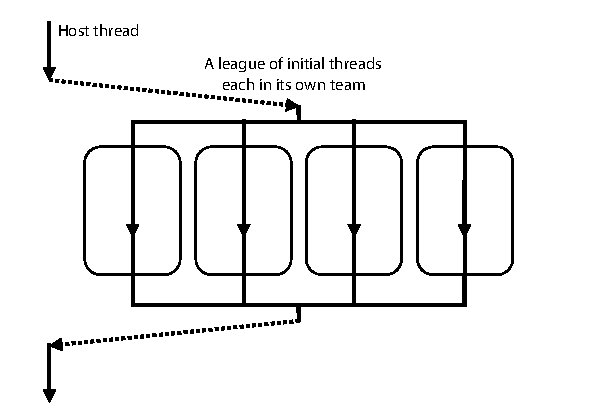
\includegraphics[clip=true,scale=1.00]
         {./06.heterogeneous_systems/figures/chapter-6-device-teams1.pdf}
     }
\caption{ \textbf{The target teams construct creates a league of initial 
               threads} -- \small
        Each initial thread is a team of one thread.  The inital threads
        execute the teams region in parallel.
        }
\label{figure:chapter6-teams-pic}
\end{figure*}

\index{Accelerators!League}
\index{Accelerators!Initial thread}
In Figure~\ref{figure:chapter6-teams-v2}, the \code{target}~\code{teams} construct again
creates a league of initial threads, but this time each initial thread
immediately encounters the \code{parallel} construct at line $7$. Each initial thread then
becomes the master of a new team of multiple threads.  The number of teams and
a thread's team number are determined by the \code{omp_get_num_teams} and
\code{omp_get_team_num} runtime functions, respectively.
\index{Accelerators!omp\_get\_team\_num}
\index{OpenMP runtime functions!omp\_get\_team\_num}
\index{Accelerators!omp\_get\_num\_teams}
\index{OpenMP runtime functions!omp\_get\_num\_teams}

\begin{figure*}[!tbh]
\begin{verbatim}
 1 #include <omp.h>
 2 extern void do_team_work(int, int, int, int);
 3 #pragma omp declare target(do_team_work)
 4 void f()
 5 {
 6   #pragma omp target teams num_teams(4)
 7   #pragma omp parallel num_threads(5)
 8   {
 9     int team = omp_get_team_num();
10     int nteams = omp_get_num_teams();
11     int tid = omp_get_thread_num();
12     int nthreads = omp_get_num_threads();
13     do_team_work(team, nteams, tid, nthreads);
14   } // End of target teams
15 }
\end{verbatim}
\caption{ \textbf {Example of a parallel construct nested in a 
                   target teams construct} -- \small
          Multiple teams of threads execute the function \texttt{do\_team\_work()}.     
         }
\label{figure:chapter6-teams-v2}
\end{figure*}

The call to the \code{omp_get_num_threads()} function at line $12$ returns the
number of threads in a team, which is $5$. The call to \code{omp_get_thread_num}
at line $11$ returns the threads number in the range $0$ to $4$.
Each thread in each team (a total of 20 threads) then calls the function
\code{do\_team\_work()} passing in the team number, the number of teams, the thread number and
the number of threads in the team.  Figure~\ref{figure:chapter6-teams-pic2} diagrams
the execution of all the threads, assuming four teams with five threads per
team.

Note that if the thread calling \code{omp_get_team_num} is in a team that was
initiated by a parallel region nested inside a teams region, the function still
returns the number of the initial thread that is the ancestor of the thread.

\index{Accelerators!League}
\begin{figure*}[!tbh]
\centering
\pdfimageresolution 400
\fbox{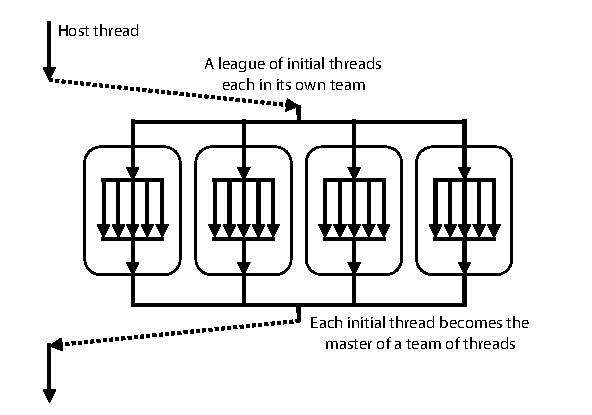
\includegraphics[clip=true,scale=1.00]
         {./06.heterogeneous_systems/figures/chapter-6-device-teams2.pdf}
     }
\caption{ \textbf{The initial threads created by the teams construct each
               become the master of a new team of threads.  } -- \small
        Each initial thread starts execution as team of one thread.  The initial threads
        execute the teams region in parallel and immediately encounter
        a parallel construct.  Each initial thread then becomes the
        master of a new team of threads.
        }
\label{figure:chapter6-teams-pic2}
\end{figure*}

%-----------------------------------------------------------------------
%------------------------- New subsection ------------------------------
%-----------------------------------------------------------------------
\subsection{The Distribute Construct}
\label{ssec:06.distribute-construct}
\index{OpenMP constructs!Distribute}
\index{Accelerators!Distribute}

\index{Accelerators!League}
\index{Accelerators!Initial thread}
The \code{target}~\code{teams} construct starts a league of initial threads where each
thread is in its own team.  Similar to the loop construct, the
\code{distribute} construct is a worksharing construct that distributes
the iterations of a loop to the initial threads in a league.  The loop
iterations are divided into chunks, which are then scheduled across the initial
threads in a league.

The \code{distribute} construct syntax in C/C++ and Fortran is shown in
Figure~\ref{figure:syntax-distribute-construct}.

\begin{figure}[!htb]
\centering
\begin{tabular}{|l|}
\hline
\ompbcdistribute \ompclauses  \\
\hspace{2em}\emph{for-loops} \\
\hline
\ompbfdistribute \ompclauses \\
\hspace{2em}\emph{do-loops} \\
\ompbfdistributeend \ompclauses \\
\hline
\end{tabular}
\caption{ \textbf{Syntax of the distribute construct in C/C++ and 
               Fortran} -- \small
          Distribute loop iterations to the initial threads in
          a league.
          }
\label{figure:syntax-distribute-construct}
\end{figure}

The clauses that are available on
the \code{distribute} construct are listed in Figure~\ref{figure:syntax-distribute-clauses}.  

\index{OpenMP clauses!private}
\index{OpenMP clauses!firstprivate}
\index{OpenMP clauses!lastprivate}
\index{OpenMP clauses!collapse}
\index{OpenMP clauses!dist\_schedule}
\index{Accelerators!Private clause}
\index{Accelerators!Firstprivate clause}
\index{Accelerators!Lastprivate clause}
\index{Accelerators!Collapse clause}
\index{Accelerators!Dist\_schedule clause}
\begin{figure*}[!tbh]
\centering
\begin{tabular}{|l|}
\hline
\bprivate \\
\bfirstprivate \\
\blastprivate \\
\bcollapse \\
\bdistschedule \\
\hline
\end{tabular}
\caption{ \textbf{Clauses supported by the distribute 
               construct} -- \small
          The dist\_schedule clause is described below.
          }
\label{figure:syntax-distribute-clauses}
\end{figure*}

Variables that appear in the \code{private}, \code{firstprivate} or
\code{lastprivate} clause are private in each initial thread.
The \code{distribute} construct has no implicit barrier at the end of the
construct.  This is like having a loop construct with a \code{nowait} clause.
The initial threads do not synchronize at a barrier at the end of the region.

The \code{collapse} clause has the same behavior as it does on the loop
construct.  It collapses the iterations of perfectly nested loops into a single
iteration space.
The restrictions on the format of the loop to which the construct applies are
the same as those for the loop construct.

How the loop iterations are scheduled to execute across the initial threads in
the league is implementation-defined, unless the \code{dist_schedule} clause is
present.
When the \code{dist_schedule(static)} clause is present, the loop iterations
are divided into contiguous chunks. If \emph{chunk\_size} appears in the
clause, then it specifies the size of the chunks.  Otherwise, each thread is
assigned no more than one chunk, and the chunks are roughly equal in size.

\index{Accelerators!League}
A version of the familiar saxpy (single precision $y=a*x+y$) function is
shown in Figure~\ref{figure:chapter6-distribute-v1}.  The \code{distribute}
worksharing construct distributes the iterations of the loop to the
initial threads in the league started by the \code{target teams} construct.

\begin{figure*}[!tb]
\begin{verbatim}
1 void saxpy(float *restrict y, float *restrict x, float a, int n)
2 {
3   #pragma omp target teams map(y[:n]) map(to:x[:n]) 
4   #pragma omp distribute
5   for (int i=0; i<n; i+=n)
6   {
7       y[i] =  y[i] + a*x[i];
8   }
9 }
\end{verbatim}
\caption{ \textbf {Example of the distribute worksharing construct} -- \small
          Each initial thread created by the target teams construct 
          executes a subset of the iterations in the loop's iteration space.
         }
\label{figure:chapter6-distribute-v1}
\end{figure*}

What is the difference between the execution of the \code{for} (or \code{do} in Fortran) and the
\code{distribute} worksharing constructs? The \code{distribute} construct has the potential
for better performance because of the restrictions on where it can be used and
what other \OMP\ constructs can appear inside the distribute region.  This
enables the compiler to be more aggressive with optimizations.  The
\code{for} and \code{do} constructs are more versatile but may not perform as well.  

The idea behind the \code{target}~\code{teams} and \code{distribute} constructs is to
spread the execution of a loop coarsely across hardware compute units and
then more finely to the threads that execute within those compute units.  What
we have shown so far is how to distribute the loop iteration to the compute
units.

The code in Figure~\ref{figure:chapter6-distribute-v2} converts the saxpy loop
into a doubly nested loop.  

\begin{figure*}[!tbh]
\begin{verbatim}
 1 void saxpy(float *restrict y, float *restrict x, float a, int n)
 2 {
 3   // Assume n is even
 4   #pragma omp target teams map(y[:n]) map(to:x[:n]) num_teams(2) 
 5   #pragma omp distribute
 6   for (int j=0; j<n; j+=n/2)
 7   {
 8     #pragma omp parallel num_threads(4)
 9     #pragma omp for
10     for (int i=j; i<n/2; i++)
11       y[i] = y[i] + a*x[i];
12   }
13 }
\end{verbatim}
\caption{ \textbf {Example of worksharing a loop across two levels of
                   parallelism} -- \small
          Use team level parallelism on the outer loop and thread level
          parallelism on the inner loop.  Distribute the loop iterations to two
          teams.  Each team then uses four threads to execute the iterations
          that are assigned to it.  
         }
\label{figure:chapter6-distribute-v2}
\end{figure*}

\index{Accelerators!League}
\index{Accelerators!Initial thread}
The \code{distribute} construct at line $5$ assigns the execution of two
iterations in the outer loop to a league of two initial threads.  The
\code{parallel} construct at line $8$ is then encountered by each initial
thread with different values for \code{j}.  Each initial thread becomes the master
thread in a team of four threads.  The first team executes the first half of
the loop iterations and the second team executes the other half.  The loop
iterations scheduled to execute on an initial thread are then scheduled
according to the \code{for} worksharing construct at line $9$, to execute on
the team of threads that the initial thread is now the master of.

In accelerated worksharing, loops are first scheduled at a coarse level to
teams and then more finely to the threads in each team.  We rewrote the saxpy
loop in order to schedule it across two levels of parallelism: teams and
threads.  However, rewriting loops is tedious and is something we want to avoid.

Section~\ref{ssec:06.composite-worksharing-loop-construct} introduces
\emph{composite} accelerated worksharing constructs.  When composite
accelerated worksharing constructs are used, loop itertions are distributed
across multiple levels of parallelism without having to rewrite the loop as we
did in Figure~\ref{figure:chapter6-distribute-v2}.  

%-----------------------------------------------------------------------
%------------------------- New subsection ------------------------------
%-----------------------------------------------------------------------
\subsection{Combined and Composite Accelerated Worksharing Constructs}
\label{ssec:06.composite-worksharing-loop-construct}
\index{Composite construct}
\index{Combined construct}
\index{Combined construct! Target}
\index{Combined construct! Target teams}
\index{Accelerators!Workshare construct}

Recall that combined constructs are short-hand notation for specifying the
individual constructs in which one construct is immediately nested inside another.
For example, the \code{parallel}~\code{for} combined construct is equivalent to
a \code{parallel} construct with a \code{for} construct nested immediately
inside the \code{parallel} construct.  The combined construct has the same
execution behavior as the two separate constructs.  However, in some instances,
depending on the compiler, the combined constructs may achieve better
performance than the individual constructs.

With some exceptions, the clauses that may appear on a combined
construct are any of the clauses that may appear on the individual
constructs that make up the combined construct.
There are many new combined
constructs involving the device constructs.  They are presented
in this section in two groups.  

The first group is the \emph{combined target} constructs.  The constructs in
this group combine the \code{target} construct with other constructs.
The second group is the \emph{combined target teams} constructs.  
They combine the \code{target teams} construct with new
worksharing constructs.  This second group is discussed at the end of this section
after the new worksharing constructs are presented.

The syntax for the combined target constructs in C/C++ and Fortran
are shown in Figure~\ref{figure:chapter6-combined-target}.  The combined
target constructs that include a \code{parallel} directive create a
team of threads where the initial thread is the master of the team.
The target simd region is executed by an initial thread that uses SIMD
parallelism to execute the iterations of the subsequent loop.

\index{OpenMP constructs!Target parallel}
\index{Accelerators!Target parallel}
\index{OpenMP constructs!Target parallel loop}
\index{Accelerators!Target parallel loop}
\index{OpenMP constructs!Target parallel loop simd}
\index{Accelerators!Target parallel loop simd}
\index{OpenMP constructs!Target simd}
\index{Accelerators!Target simd}
\begin{figure}[!htbp]
\centering
\begin{tabular}{|l|}
\hline
\ompbctargetparallel \ompclauses \\
\hspace{2em}\emph{structured block} \\
\hline
\ompbctargetparallelfor \ompclauses \\
\hspace{2em}\emph{for-loops} \\
\hline
\ompbctargetparallelforsimd \ompclauses \\
\hspace{2em}\emph{for-loops} \\
\hline
\ompbctargetsimd \ompclauses \\
\hspace{2em}\emph{for-loops} \\
\hline
\hline
\ompbftargetparallel \ompclauses \\
\hspace{2em}\emph{structured block} \\
\ompbftargetparallelend \ompclauses \\
\hline
\ompbftargetparalleldo \ompclauses \\
\hspace{2em}\emph{do-loops} \\
\ompbftargetparalleldoend \ompclauses \\
\hline
\ompbftargetparalleldosimd \ompclauses \\
\hspace{2em}\emph{do-loops} \\
\ompbftargetparalleldosimdend \ompclauses \\
\hline
\ompbftargetsimd \ompclauses \\
\hspace{2em}\emph{do-loops} \\
\ompbftargetsimdend \ompclauses \\
\hline
\end{tabular}
\caption{ \textbf{Syntax of the combined target constructs in C/C++ and Fortran} -- \small
          Constructs combining \texttt{target} with other constructs.  A \texttt{copyin}
          clause may not appear on any of the combined target constructs.
          }
\label{figure:chapter6-combined-target}
\end{figure}

A composite construct is different than a combined construct.  
Composite constructs combine multiple constructs, but the combination has
execution behavior that is different from when the constructs are specified
separately.  

\index{Accelerators!League}
\index{Accelerators!Initial thread}
The \code{distribute}~\code{parallel}~\code{for} construct is a composite
accelerated worksharing construct that distributes the iterations of a loop
across two levels of parallelism.  Each initial thread in the league that
encounters the construct becomes the master thread of a team.  The iterations
of a loop are first distributed to the master threads.  The subset of loop
iterations assigned to the master thread are then again distributed to the
threads in the team.

The code in Figure~\ref{figure:chapter6-distribute-v3} shows how the
~\code{distribute}~\code{parallel}~\code{for} accelerated worksharing
construct is used to distribute the iterations of the saxpy loop to 
teams and then to the threads in those teams.

Another way to look at this type of construct is to consider the nested version
of the C/C++ saxpy loop from Figure~\ref{figure:chapter6-distribute-v2}.  We had
to rewrite the loop to distribute its iterations across two levels of
parallelism.

The \code{distribute}~\code{parallel}~\code{for} (or
\code{distribute}~\code{parallel}~\code{do} in Fortran) construct tells the
compiler to create the second level of parallelism and to distribute loop
iterations across the two levels of parallelism.  So, now we don't have to
rewrite loops!

\begin{figure*}[!tbh]
\begin{verbatim}
1 void saxpy(float *restrict y, float *restrict x, float a, int n)
2 {
3   #pragma omp target teams map(y[:n]) map(to:x[:n]) 
4   #pragma omp distribute parallel for
5   for (int i=0; i<n; i++)
6     y[i] = y[i] + a*x[i];
7 }
\end{verbatim}
\caption{ \textbf {Example of the distribute parallel loop accelerated 
                   worksharing construct} -- \small
          Create multiple thread teams executing in parallel.
          Distribute loop iterations to the teams and then
          to the threads in each team.
         }
\label{figure:chapter6-distribute-v3}
\end{figure*}

\index{Accelerators!League}
\index{Accelerators!Initial thread}
The first level of parallelism is created by a \code{target}~\code{teams} construct.  When
the resulting league of initial threads encounters
the \code{distribute}~\code{parallel}~\code{loop} construct, the following steps occur:
\begin{enumerate}

\item By the \code{distribute} part of the construct, each initial thread is
assigned loop iterations according to the \code{distribute} construct's
scheduling algorithm.

\item By the \code{parallel} part of the construct, each initial thread becomes
the master thread of a thread team.  This creates the second level of
parallelism. Now multiple teams of threads are
executing in parallel.

\item By the \code{for} part of the construct, the subset of iterations
assigned to each initial thread (the master thread) are then distributed across
the threads in each team.

\end{enumerate}

The composite accelerated worksharing constructs and their syntax in C/C++ and
Fortran are shown in Figure~\ref{figure:chapter6-accel-work-sharing-construct}.
With a few exceptions, all clauses that may appear on the individual directives
that make up the construct, may appear on the composite construct.

\index{OpenMP constructs!Distribute parallel loop}
\index{Accelerators!Distribute parallel loop}
\index{OpenMP constructs!Distribute simd}
\index{Accelerators!Distribute simd}
\index{OpenMP constructs!Distribute parallel loop simd}
\index{Accelerators!Distribute parallel loop simd}
\begin{figure}[!htbp]
\centering
\begin{tabular}{|l|}
\hline
\ompbcdistributeparallelfor \ompclauses  \\
\hspace{2em}\emph{for-loops} \\
\hline
\ompbcdistributesimd \ompclauses  \\
\hspace{2em}\emph{for-loops} \\
\hline
\ompbcdistributeparallelforsimd \ompclauses  \\
\hspace{2em}\emph{for-loops} \\
\hline
\hline
\ompbfdistributeparalleldo \ompclauses \\
\hspace{2em}\emph{do-loops} \\
\ompbfdistributeparalleldoend \ompclauses \\
\hline
\ompbfdistributesimd \ompclauses \\
\hspace{2em}\emph{do-loops} \\
\ompbfdistributesimdend \ompclauses \\
\hline
\ompbfdistributeparalleldosimd \ompclauses \\
\hspace{2em}\emph{do-loops} \\
\ompbfdistributeparalleldosimdend \ompclauses \\
\hline
\end{tabular}
\caption{ \textbf{Syntax of the composite accelerated worksharing constructs 
               in C/C++ and Fortran} -- \small
          Distribute loop iterations across multiple levels of
          parallelism: teams, threads and SIMD lanes.
          }
\label{figure:chapter6-accel-work-sharing-construct}
\end{figure}

The \code{distribute}~\code{simd} construct distributes loop iterations across
two levels of parallelism.  Loop iterations are assigned to the initial
threads in a league according to the \code{distribute} constructs scheduling
algorithm.  Each initial thread then uses SIMD parallelism to execute
the loop iterations assigned to it.

The \code{distribute}~\code{parallel}~\code{for}~\code{simd} (or
\code{distribute}~\code{parallel}~\code{do}~\code{simd} in Fortran)  construct
distributes loop iterations across three levels of parallelism.  Loop
iterations are first assigned to the initial threads in each team.  Each
initial thread becomes the master of a new team of threads.  The loop
iterations assigned to an initial thread are then distributed to the threads in
the master thread's team.  Each thread then uses SIMD parallelism to execute
the iterations assigned to it.

The composite accelerated worksharing constructs may be combined with the
\code{target teams} construct.  As mentioned at the beginning of this section,
these are called combined target teams constructs.  The combined target teams
constructs and their syntax in C/C++ and Fortran are shown in
Figure~\ref{figure:chapter6-combined-teams}.  
%Some of them are quite long.

\index{Combined construct!Target teams}
\index{OpenMP constructs!Target teams distribute simd}
\index{Accelerators!Target teams distribute simd}
\index{OpenMP constructs!Target teams distribute}
\index{Accelerators!Target teams distribute}
\index{OpenMP constructs!Target teams distribute parallel loop}
\index{Accelerators!Target teams distribute parallel loop}
\index{OpenMP constructs!Target teams distribute parallel loop simd}
\index{Accelerators!Target teams distribute parallel loop simd}
\begin{figure}[!htbp]
\centering
\begin{tabular}{|l|}
\hline
\ompbctargetteamsdistribute \ompclauses \\
\hspace{2em}\emph{for-loops} \\
\hline
\ompbctargetteamsdistributeparallelfor \ompclauses \\
\hspace{2em}\emph{for-loops} \\
\hline
\ompbctargetteamsdistributesimd \ompclauses \\
\hspace{2em}\emph{for-loops} \\
\hline
\ompbctargetteamsdistributeparallelforsimd{ \emph{[clause[[,]\ldots}}\\
\hspace{2em}\emph{for-loops} \\
\hline
\hline
\ompbftargetteamsdistribute \ompclauses \\
\hspace{2em}\emph{do-loops} \\
\ompbftargetteamsdistributeend \\
\hline
\ompbftargetteamsdistributeparalleldo \ompclauses \\
\hspace{2em}\emph{do-loops} \\
\ompbftargetteamsdistributeparalleldoend \\
\hline
\ompbftargetteamsdistributesimd \ompclauses \\
\hspace{2em}\emph{do-loops} \\
\ompbftargetteamsdistributesimdend \\
\hline
\ompbftargetteamsdistributeparalleldosimd \ompclauses \\
\hspace{2em}\emph{do-loops} \\
\ompbftargetteamsdistributeparalleldosimdend \\
\hline
\end{tabular}
\caption{ \textbf{Syntax of the combined target teams constructs in C/C++ and Fortran} -- \small
          Constructs that combine \texttt{target teams} and accelerated worksharing constructs.
          }
\label{figure:chapter6-combined-teams}
\end{figure}

\index{Combined construct!Target teams reduction}
Because the \code{target teams} construct is a combined construct, 
the \code{target} construct may be separated out of 
a combined target teams construct (see Section~\ref{sec:06.teams-construct}).
For example, a \code{target teams distribute} construct may be separated into a
\code{target} construct with an immediately nested \code{teams
distribute} construct.  Typically, this is simply a syntax preference, but
there are some instances when \code{target} must be a separate construct.
This can occur when a variable must be \code{private} in the teams region and
mapped in the target region.  

A variable cannot appear in both a \code{map} clause and a data-sharing
attribute clause on the same
construct.  For example, in Figure~\ref{figure:chapter6-targetteams-reduction}
the variable \code{sum} appears in a \code{reduction} clause, and therefore, cannot also
appear in a \code{map} clause.  Because \code{sum} is not mapped, its reduced value is 
lost after the \code{target teams} region completes.\footnote{The same problem
can occur when using a \code{reduction} clause on the target combined constructs.}

\begin{figure*}[!tbh]
\begin{verbatim}
 1 int dotp(int *restrict a, int *restrict b, int n)
 2 {
 3   int sum = 0;
 4 
 5   #pragma omp target teams distribute map(to:a[:n],b[:n]) \
 6                                       reduction(+:sum)
 7   for (int i=0; i<n; i++)
 8     sum += a[i] * b[i];
 9 
10   return sum;  // Sum is always 0
11 }
\end{verbatim}
\caption{ \textbf {A variable cannot appear in both map and reduction clauses on the same construct} -- \small
          The \texttt{reduction} clause is associated with the
          \texttt{teams} directive.
          The variable \texttt{sum} is not mapped, and therefore,
          the reduced value of \texttt{sum} is lost after the region.
        }
\label{figure:chapter6-targetteams-reduction}
\end{figure*}

The solution, as shown in
Figure~\ref{figure:chapter6-targetteams-reduction-v2}, is to use a separate
\code{target} construct that explicitly maps the variable \code{sum}.  Each initial
thread that executes the teams region gets a private instance of \code{sum}.  Once
the teams region is complete, the mapped \code{sum} variable contains the reduced
value.  In the map-exit phase for the target region, the reduced value
is assigned to the host's original \code{sum} variable. 

\begin{figure*}[!tbh]
\begin{verbatim}
 1 int dotp(int *restrict a, int *restrict b, int n)
 2 {
 3   int sum = 0;
 4 
 5   #pragma omp target map(sum) map(to:a[:n],b[:n])
 6   #pragma omp teams distribute reduction(+:sum)
 7   for (int i=0; i<n; i++)
 8     sum += a[i] * b[i];
 9 
10   return sum;
11 }
\end{verbatim}
\caption{ \textbf {Use a separate target construct to map reduction variables} -- \small
          The variable \texttt{sum} is private in the teams region, but now mapped
          in the target region.
        }
\label{figure:chapter6-targetteams-reduction-v2}
\end{figure*}


%-----------------------------------------------------------------------
%------------------------- New section ---------------------------------
%-----------------------------------------------------------------------
\section{Data Mapping Clauses}
\label{sec:06.data-mapping-clauses}

\index{Accelerators!Device data environment}
\index{Device data environment}
Recall from Section~\ref{ssec:06.device-data-environments} that an accelerator has a
\emph{device data environment}, which contains the set of all variables that are
available to the threads executing on that accelerator.  When an 
\emph{original}~\emph{variable} in the host's data environment is mapped to an accelerator, a
\emph{corresponding}~\emph{variable} is allocated in the accelerator's device data
environment.  During the execution of a program, the set of corresponding
variables in an accelerator's device data environment will change as variables
are mapped and unmapped from it.

Depending on the memory architecture of the heterogeneous system, the original
and corresponding variables may or may not share the same storage location.
Because of this, a user must consider these two aspects of mapped
variables: \begin{itemize}

    \item Because the original and corresponding variables \emph{may} share the
    same storage location, a mapped variable should be thought of like a shared
    variable.  This means that if either the original or the corresponding
    variable is written to by a thread, synchronization and memory consistency
    operations are required to avoid data races.

    \item Because the original and corresponding variables \emph{may not} share
    the same storage location, copy operations might be required to make the
    original and corresponding variables consistent.  These copy operations can
    be costly in regards to performance and should be
    avoided if possible.

\end{itemize}

If a variable is accessed in a target
region, but the variable does not appear as a list item in a \code{map} clause
on the construct then there are default rules to determine if the variable is
mapped or private.  These rules and the \code{defaultmap} clause are covered in
Section~\ref{ssec:06.defaultmap-clause}.  Structure members may appear as list
items in a \code{map} clause but with some limitations that are described in
Section~\ref{ssec:06.map-structs}.
Section~\ref{ssec:06.zero-array-sections} shows how to access
previously mapped memory using pointer-based array sections with a length of
zero.

%Section~\ref{ssec:06.zero-array-sections} covers what happens when an
%array section with a length of zero appears in a \code{map} clause.


%-----------------------------------------------------------------------
%------------------------- New subsection ------------------------------
%-----------------------------------------------------------------------
\subsection{The Map Clause}
\label{sec:06.map-clause}
\index{OpenMP clauses!map}
\index{Accelerators!Map clause}

\index{Accelerators!Array section}
\index{Array section}
Variable names, array sections, and structure elements may appear as list items
in a \code{map} clause.  An optional \emph{map-type} and \code{always}
\emph{map-type-modifier} control how the list items are mapped.  The syntax of
the \code{map} clause is shown in Figure~\ref{figure:syntax-map-clause}.  If no
\emph{map-type} is specified, the default is \code{tofrom}.

\index{Mapped variable}
\index{Mapped variable!Map-type}
\index{Mapped variable!Alloc map-type}
\index{Mapped variable!To map-type}
\index{Mapped variable!Delete map-type}
\index{Mapped variable!From map-type}
\index{Mapped variable!Release map-type}
\index{Mapped variable!Tofrom map-type}
\index{Mapped variable!Always map-type-modifier}
\begin{figure}[!b]
\centering
\begin{tabular}{|l|}
\hline
\code{map} \emph{([[map-type-modifier[,]] map-type:] list)} \\
\hline
where the optional \emph{map-type} is one of:  \\
\hspace{2em}\code{alloc} \\
\hspace{2em}\code{to} \\
\hspace{2em}\code{from} \\
\hspace{2em}\code{tofrom} \\
\hspace{2em}\code{release} \\
\hspace{2em}\code{delete} \\
\hline
where the optional \emph{map-type-modifier} is:  \\
\hspace{2em}\code{always} \\
\hline
\end{tabular}
\caption{ \textbf{Syntax of the map clause in C/C++ and Fortran} -- \small
          The map clause controls how variables are mapped.
          }
\label{figure:syntax-map-clause}
\end{figure}

\index{Mapped variable!Map-enter phase}
\index{Mapped variable!Map-exit phase}
There are three phases that occur when mapping a variable in a \code{target}
region: \begin{enumerate}
    \item The \emph{map-enter} phase occurs on entry to the \code{target}
    region when the variable is mapped to the accelerator.  
    \item The \emph{compute} phase occurs when, during the execution of the
    \code{target} region, threads executing on the accelerator access the
    mapped variable.
    \item The \emph{map-exit} phase occurs on exit from a \code{target} region
    when the variable is unmapped from the accelerator.  
\end{enumerate}

The map-enter and map-exit phases manage the storage allocation and copy
operations for a mapped variable.
In the map-enter phase storage is allocated for the variable in the accelerator's
address space, and then the value of host's original variable is copied to the 
accelerator's corresponding variable.
In the map-exit phase, the value of the accelerator's corresponding variable 
is copied to the host's original variable, and then the storage for the 
corresponding variable in the accelerator's address space is released.
    
%The map-enter and map-exit phases manage the storage allocation and copy
%operations for a mapped variable as follows:
%
%In the map-enter phase: \begin{list}
%  \item Allocate storage for the corresponding variable in the accelerator's
%  address space.
%  \item Copy the value of the host's original variable to the accelerator's
%  corresponding variable.
%\end{list}
%
%  \item compute phase: \begin{itemize}
%    \item Threads running on the accelerator access the corresponding variable
%    during the execution of a target region.
%  \end{itemize}
%
%In the map-exit phase: \begin{enumerate}
%  \item Copy the value of the accelerator's corresponding variable to the
%  host's original variable.
%  \item Release the storage for the corresponding variable in the accelerator's
%  address space.
%\end{enumerate}

In Figure~\ref{figure:chapter6-map-v1}, the map-enter phase occurs on entry to
the target region at line $3$.  Storage is allocated for the three
corresponding arrays \code{a}, \code{b} and \code{t} in the accelerator's address space.  The
values of the host's original \code{a}, \code{b} and \code{t} array variables are then copied
to the accelerator's corresponding array variables. 

\begin{figure*}[!b]
\begin{verbatim}
 1 #include <stdlib.h>
 2 void func(float a[1024], float b[1024], int t[1024])
 3 {
 4   #pragma omp target map(a, b, t) // Map-enter
 5   {
 6     int i;
 7 
 8     for (i=0; i<1024; i++)
 9       t[i] = rand()%1024;
10 
11     for (i=0; i<1024; i++)
12       a[i] =  b[t[i]];
13 
14   } // End of target, map-exit
15 }
\end{verbatim}
\caption{ \textbf {Example of the map clause} -- \small
          Copies occur for the arrays \texttt{a}, \texttt{b}, and 
          \texttt{t} at the entry to and exit from the target region.
         }
\label{figure:chapter6-map-v1}
\end{figure*}

The map-exit occurs on exit from the target region at line $14$.  The values of
the accelerator's corresponding array variables are copied back to the host's
original array variables, and the storage for the three variables in the
accelerator's address space is then released.

Notice that, in the compute phase, the arrays \code{a} and \code{t} are only written to and
that array \code{b} is only read from.  Let's assume that \code{t} is a temporary variable, and
that the values written to it are never used after the target region.  It is
apparent then that the copies for \code{a} and \code{c} that occur during the map-enter
phase are not needed.  Further, the copies that occur during the map-exit phase
for \code{b} and \code{c} are not needed.  

\index{Mapped variable!Map-enter phase}
\index{Mapped variable!Map-exit phase}
The \code{map} clause's \emph{map-type} is used to optimize the copies that
occur during the map-enter and map-exit phases. On many heterogeneous systems,
it is costly to copy variables between the host and an accelerator.  The
\emph{map-type} is used to disable these copies as shown in
Figure~\ref{figure:chapter6-map-types}.

\index{Mapped variable}
\index{Mapped variable!Map-type}
\index{Mapped variable!Alloc map-type}
\index{Mapped variable!To map-type}
\index{Mapped variable!Delete map-type}
\index{Mapped variable!From map-type}
\index{Mapped variable!Release map-type}
\index{Mapped variable!Tofrom map-type}
\begin{figure*}[!b]
\centering
\begin{tabular}{|l l l|}
\hline
\code{map-type} & Perform map-enter copies & Perform map-exit copies \\
\hline
\code{alloc} & No & No \\
\code{to} & Yes & No \\
\code{from} & No & Yes \\
\code{tofrom} & Yes & Yes \\
\code{release} & -- & No \\
\code{delete} & -- & No \\
\hline
\end{tabular}
\caption{ \textbf{Map-type effect on mapping variables} -- \small
          The default \emph{map-type} is \texttt{tofrom}.  The \texttt{release}
          and \texttt{delete} \emph{map-types} apply only to the map-exit phase
          and can only appear in a \texttt{map} clause on a
          \texttt{target}~\texttt{exit}~\texttt{data} construct (See
          Section~\ref{ssec:06.target-enter-and-exit-data-constructs}).
        }
\label{figure:chapter6-map-types}
\end{figure*}

In Figure~\ref{figure:chapter6-map-v2} the code from
Figure~\ref{figure:chapter6-map-v1} is updated to use explicit map-types.  The
map-enter phase occurs on entry to the target region at line $4$ and
storage is allocated for the three corresponding arrays \code{a}, \code{b} and \code{t} in the
accelerator's address space.  Only the value of the host's original \code{b} array
variable is copied to the accelerator's corresponding \code{b} array variable. The
corresponding \code{a} and \code{t} array variables are left uninitialized.  The map-exit
phase occurs on exit from the target region at line $15$.  Only the
value of the accelerator's corresponding \code{a} array variable is copied to the
host's original \code{a} array variable.  The storage in the accelerator's address
space for all three variables is then released.  Using map-types, unnecessary
copy operations have been eliminated.

\begin{figure*}[!tb]
\begin{verbatim}
 1 #include <stdlib.h>
 2 void func(float a[1024], float b[1024], int t[1024])
 3 {
 4   #pragma omp target map(from:a) map(to:b) \
 5                      map(alloc:t) // Map-enter
 6   {
 7     int i;
 8 
 9     for (i=0; i<1024; i++)
10       t[i] = rand()%1024;
11 
12     for (i=0; i<1024; i++)
13       a[i] =  b[t[i]];
14 
15   } // End of target, map-exit
16 }
\end{verbatim}
\caption{ \textbf {Example of the map clause with map-types} -- \small
          Eliminate superfluous copies by using map-types.
         }
\label{figure:chapter6-map-v2}
\end{figure*}

On entry to a \code{target}, \code{target}~\code{data}, or
\code{target}~\code{enter}~\code{data} construct, a map-enter phase occurs.
Likewise, on exit from a \code{target}, \code{target}~\code{data}, or
\code{target}~\code{exit}~\code{data} construct, a map-exit phase occurs.
The \code{target}~\code{data}, \code{target}~\code{enter}~\code{data}, and
\code{target}~\code{exit}~\code{data} data mapping constructs only map
variables and do not execute any code on an accelerator (see
Section~\ref{sec:06.data_mapping_constructs}).

What happens when a construct maps a variable, but that variable has already
been mapped by a \code{target}~\code{enter}~\code{data} construct or by an
enclosing \code{target}~\code{data} construct?  
There can be only one instance of a corresponding variable in an accelerator's
device data environment.  A reference count is associated with each
corresponding variable.  When a variable is \emph{present} in an accelerator's
device data environment, its corresponding variable's reference count is
greater than or equal to one.
The map-enter and map-exit phases increment or decrement the
corresponding variable's reference count.  The point of the reference count is
to keep track of the number of times a variable has been mapped and to only
remove it from the accelerator device data environment after it has been
unmapped the same number times.

In the code in
Figure~\ref{figure:chapter6-map-v3} 
\code{target}~\code{data} construct at line $5$ maps the variables \code{a}, \code{b} and
\code{t} according to their respective map-types.  
However, the variables \code{a}, \code{b} and \code{t}
are mapped again by the enclosed \code{target} constructs at lines $8$ and $16$.

\begin{figure*}[!tb]
\begin{verbatim}
 1 #include <stdlib.h>
 2 #include <stdio.h>
 3 void func(float a[1024], float b[1024], int t[1024])
 4 {
 5   #pragma omp target data map(from:a) map(to:b) \
 6                           map(alloc:t) // Map-enter
 7   {
 8     #pragma omp target map(always,from:t) // Map-enter
 9     for (int i=0; i<1024; i++) {
10       t[i] = rand()%1024;
11     } // Map-exit
12 
13     for (int i=0; i<1024; i++)
14        printf("t[%d]=%d\n", i, t[i]);
15 
16     #pragma omp target map(a,b,t) // Map-enter
17     for (int i=0; i<1024; i++) {
18       a[i] =  b[t[i]];
19     } // Map-exit
20 
21   } // End of target data, map-exit
22 }
\end{verbatim}
\caption{ \textbf {Example of a variable appearing in nested map clauses} -- \small
          There is only one instance of a variable in an accelerator's
          address space.
         }
\label{figure:chapter6-map-v3}
\end{figure*}

The \code{target}~\code{data} construct's map-enter phase at line $5$ allocates
storage in the accelerator's address space for the variables \code{a}, \code{b} and \code{t}.
Only the corresponding variable \code{a} is assigned the value of the host's
original \code{a} variable.  The \code{b} and \code{t} corresponding variables are
uninitialized.

\index{Mapped variable}
\index{Mapped variable!Map-type}
\index{Mapped variable!Always map-type-nodifier}
The target construct's map-enter phase at line $8$ does not allocate storage
for the variable \code{t}, because \code{t} is already present in the accelerator's device
data environment.  The \code{always} \emph{map-type-modifier} combined with the
\code{from} \emph{map-type} forces a copy of \code{t} from the accelerator to the host
during the map-exit phase at the end of the target region at line $11$.

\index{Mapped variable!Map-enter phase}
The target construct's map-enter phase at line $16$ does not allocate storage
or copy the variables \code{a}, \code{b} and \code{t} to the accelerator, because they are
already present in the accelerator's device data environment.  Likewise, the
map-exit phase at line $19$ does not copy the variables back to the host or
release the storage on the accelerator.  In this case, it is as if the effects
of the \code{map} clause are ignored.

\index{Mapped variable!Map-exit phase}
Finally, at line $20$ the map-exit phase for the \code{target}~\code{data}
construct copies the value of the \code{b} from the accelerator and then releases
the storage for all three variables.

%To briefly review, the map-enter phase for a variable includes two conditional
%actions: 1) storage allocation and 2) a copy operation to the accelerator.
%Likewise, the map-exit phase for a variable includes the following two conditional actions: 1)
%a copy operation from the accelerator and 2) storage release.  

%The allocation and release of storage actions are  conditioned to occur based
%on the reference count.  Further, the copy operations are conditioned to occur
%depending on the \emph{map-type} and \code{always} \emph{map-type-modifier}.

At the start of the map-enter phase, if a corresponding variable's
reference count is greater than or equal to one, then no new storage is allocated,
and the value of the original variable is not copied to the corresponding
variable.  The only effect is that the reference count is incremented.

Likewise, at the start of a map-exit phase, if a corresponding variable's
reference count is greater than one, then the value of the corresponding
variable is not copied back to the original variable, and its storage is not
released.  The only effect is that the reference count is decremented.

%In the map-enter phase, when a mapped variable's map-type is \code{to} or
%\code{tofrom}, a copy to a corresponding variable occurs only when the
%reference count is incremented to one (such as when the corresponding variable is
%entered into the accelerator's data environment).

%Similarly, in the map-exit phase, when a mapped variable's map-type is
%\code{from} or \code{tofrom}, a copy from a corresponding variable
%only occurs when the reference count is decremented to zero (such as when the corresponding
%variable is removed from the accelerator's device data environment).

The \code{always} \emph{map-type-modifier} asserts that the map-enter and
map-exit copies should occur regardless of the reference count.  It
provides a way to force a copy to occur.

\index{Mapped variable}
\index{Mapped variable!Map-type}
\index{Mapped variable!Alloc map-type}
\index{Mapped variable!To map-type}
\index{Mapped variable!Delete map-type}
\index{Mapped variable!From map-type}
\index{Mapped variable!Release map-type}
\index{Mapped variable!Tofrom map-type}
\index{Mapped variable!Always map-type-nodifier}
The steps associated with the map-enter and map-exit phases are updated to
incorporate the reference count, \emph{map-type}, and \emph{map-type-modifier}
as shown below:

The map-enter phase: \begin{enumerate}

  \item If a corresponding variable is not present in the accelerator's device
  data environment then: \begin{itemize}
     
    \item Allocate storage in the accelerator's address space for the
    corresponding variable, and initialize its reference count to zero.

  \end{itemize}

  \item Increment the corresponding variable's reference count by one.

  \item If the \code{to} or \code{tofrom} map-type is specified then:
  \begin{itemize}

    \item If the corresponding variable's reference count is one or the
    \code{always} \emph{map-type-modifier} is specified, then assign the value of the
    host's original variable to the accelerator's corresponding variable.

  \end{itemize}

\end{enumerate}

The map-exit phase: \begin{itemize}

  \item If a corresponding variable is present in the accelerator's device
  data environment then: \begin{enumerate}

    \item If the \code{from} or \code{tofrom} \emph{map-type} is specified
    then: \begin{itemize} 
    
      \item If the corresponding variable's reference count is one or the
      \code{always} \emph{map-type-modifier} is specified, then assign the value
      of the accelerator's corresponding variable to the
      host's original variable.

    \end{itemize}

    \item Decrement the corresponding variable's reference count by one.

%    \item If the \code{delete} \emph{map-type} is specified, then set the
%    corresponding variable's reference count to zero.

    \item If the \code{delete} \emph{map-type} is specified and the
    corresponding variable's reference count is not infinite, then
    set it to zero.

    \item If the corresponding variable's reference count is zero, then release the storage
    for the corresponding variable in the accelerator's address space.

  \end{enumerate}

\end{itemize}

Although the \code{alloc} and \code{release} \emph{map-types} do not appear
explicity above, their effect is to either decrement or increment the reference count.  
The \code{delete} \emph{map-type} sets the reference count to zero.  It
provides a way to force the removal of a variable from an accelerator's device
data environment.  
Globally mapped variables and device memory associated to host memory by the
\code{omp_target_associate_ptr()} function have an infinite reference count and
cannot be removed.
Both the \code{delete} and \code{release} \emph{map-types}
may appear only in \code{map} clauses on the
\code{target}~\code{exit}~\code{data} construct (see Section~\ref
{ssec:06.target-enter-and-exit-data-constructs}).
\index{Accelerators!omp\_target\_associate\_ptr} 
\index{OpenMP runtime functions!omp\_target\_associate\_ptr} 
\index{Mapped variable!Globally mapped}

%-----------------------------------------------------------------------
%------------------------- New subsection ------------------------------
%-----------------------------------------------------------------------
\subsection{Mapping Structure Members}
\label{ssec:06.map-structs}
\index{OpenMP clauses!map}
\index{Accelerators!Map clause}
\index{Mapped variable!Structure member}

Similar to how an array section can map a subset of the elements in an array,
individual structure members can appear in \code{map} clauses in order to map
a subset of the members in a structure variable.  The restrictions on mapping
structure members are as follows:

\begin{itemize}

 \item Structure members must explicitly appear in \code{map} clauses,
 otherwise a reference to a structure member in a \code{target} construct
 implicitly maps the whole structure.

 \item To map a subset of the members in a structure variable, 
 all structure members in the subset must appear in a \code{map} clause(s) on the same
 construct.

 \item If a subset of members of a structure variable are mapped, only the
 structure members in the subset can be referenced in a \code{target} region.

 \item When a subset of members of a structure variable are mapped, the
 subset may not be increased by additionally mapping other members of the
 structure variable.

 \item C/C++ structure members with type pointer may appear as the base of an
 array section, but only the rightmost structure member can specify an array
 section.  For example, \code{S.a[:100]} is legal syntax, but \code{S.b[:100].z} is not.
 \index{Mapped variable!Array section}
 \index{Array section!Pointer-based}
 \index{Array section!Structure member}

\end{itemize}

\index{Accelerators!Mapped function}
To illustrate these concepts, some simple use cases are presented in
Figure~\ref{figure:chapter6-mapstruct}.  A structure type \code{Stype} is declared
at line $1$. Lines $3-4$ use the \code{declare}~\code{target} construct to declare that
\code{f1()}, \code{f2()}, and \code{f3()} are mapped functions and may be called from a target region 
(see Section~\ref{sec:06.declare-target-construct}).

\begin{figure*}[!tb]
\begin{verbatim}
 1 typedef struct { int x, y, size, *p; } Stype;
 2 extern Stype S;
 3 extern int f1(int,int), f2(int*,int), f3(Stype *);
 4 #pragma omp declare target to(f1, f2, f3) 
 5 
 6 void foo1(Stype S)
 7 {
 8    #pragma omp target
 9    f1(S.x, S.y);
10 
11    #pragma omp target map(S.x, S.y)
12    f1(S.x, S.y);
13 
14    #pragma omp target map(S, S.p[:S.size])
15    f2(S.p, S.size);
16 
17    #pragma omp target map(S.x)
18    f3(&S);
19 
20    #pragma omp target data map(S.x)
21    {
22       #pragma omp target map(S.y) // Error
23       f1(S.x, S.y);
24    }
25 }
\end{verbatim}
\caption{ \textbf {Example of mapping structure members} -- \small
          Structure members may appear in map clauses and array sections with some
          restrictions.
         }
\label{figure:chapter6-mapstruct}
\end{figure*}

For the \code{target} construct at line $8$, the whole structure variable $S$
is mapped even though only the members \code{S.x} and \code{S.y} are referenced in the
construct.  The structure members \code{S.x} and \code{S.y} appear explicitly in
a \code{map} clause on the \code{target} construct at line $11$, and now only
these two members are mapped instead of the whole structure variable \code{S}.  The
\code{map} clause on the \code{target} construct at line $14$ has an array
section where \code{S.p} is used as the base of the array section.

On line $17$, only \code{S.x} is mapped, but the call at line $18$ refers to the
address of \code{S}.  This is allowed as long as the code inside the function \code{f3()}
accesses only \code{S.x}.  In the last example that spans lines $20-24$ the structure
member \code{S.x} is mapped by the \code{target}~\code{data} construct at line
$20$.  The \code{target} construct then maps \code{S.y}.  This is an error because
it tries to change the subset of mapped structure members (the fourth
restriction above).  This may be remedied by adding \code{S.y} to the \code{map}
clause on line $20$.

%-----------------------------------------------------------------------
%------------------------- New subsection ------------------------------
%-----------------------------------------------------------------------
\subsection{The Defaultmap Clause and Data-mapping Attributes}
\label{ssec:06.defaultmap-clause}
\index{OpenMP clauses!defaultmap}
\index{Accelerators!Defaultmap clause}

\index{Mapped variable!Data-mapping attribute}
If and how a variable is mapped is determined by the variable's data-mapping
attributes.  
%If a variable is not mapped in a \code{target} construct, it is
%\code{private} or \code{firstprivate}.  
The rules for determining the
data-mapping attributes for a variable are either explicitly or implicitly
determined.

\index{Mapped variable}
\index{Mapped variable!Map-type}
\index{Mapped variable!Default map-type}
The data-mapping attributes for variables that appear in clauses or are
declared in a scope inside the \code{target} construct are explicitly determined
according to the following rules: \begin{itemize}

  \item A variable that appears in a \code{map} clause is mapped according to
  the \emph{map-type}.

  \item A variable that appears in a \code{private}, \code{firstprivate}, or
  \code{is_device_ptr} clause is private.

  \item A variable that is declared in a scope inside the \code{target}
  construct is private.

\end{itemize}

The data-mapping attributes for all other variables referenced in a
\code{target} construct are implicitly determined according to the following
rules: \begin{itemize}

  \item If the variable is not a scalar variable, the variable is mapped
  with a \emph{map-type} of \code{tofrom}.

  \item If the \code{target} construct does not have a
  \code{defaultmap(tofrom:scalar)} clause, then a \emph{scalar} variable is
  \code{firstprivate}.  

  \item If the \code{target} construct has a \code{defaultmap(tofrom:scalar)}
  clause, then a \emph{scalar} variable is mapped with a \emph{map-type} of
  \code{tofrom}.

  \index{Array section!Pointer-based}
  \item A pointer variable that appears in a pointer based array section in
  C/C++ is \code{private}.

\end{itemize}

\index{Mapped variable!Scalar}
In general, variables with implicitly determined data-mapping attributes are
treated as if they had appeared in a \code{map} clause with a \emph{map-type}
of \code{tofrom}.  The exception is scalar and C/C++ pointer variables.
Scalar variables have a base language built-in type (for example, \code{int} or
\code{float} in C/C++).\footnote{The precise definition of a scalar variable is
determined by the base language.}  

The performance overhead of a mapped variable can be higher than a \code{private}
variable.  A mapped variable requires a presence check to see if the variable
is already present in the accelerator's device data environment.
Variables that are \code{private} do not require this check.  
The overhead of performing the presence
check is more pronounced for the smaller variables, such as scalars.  For these reasons,
the implicit data-sharing attribute for scalar variables referenced in a
\code{target} construct is \code{firstprivate}.  However, the
\code{defaultmap(tofrom:scalar)} clause is provided to change the implicit
data-mapping attribute for these variables to mapped with a \emph{map-type} of
\code{tofrom}.

%In addition, many implementations use something similar to a remote procedure
%call to start a target region executing on an accelerator.  It is very
%efficient to pass scalar variables by value as arguments to the remote
%procedure.  Passing arguments by value happens to match quite nicely to the
%semantics of firstprivate.

\index{Accelerators!Initial thread}
\index{Array section}
In the \code{saxpy()} function shown in Figure~\ref{figure:chapter6-defaultmap-v1}, the
scalar variables \code{a} and \code{n} are \code{firstprivate}.  
%The pointer variables $y$ and
%$x$ are \code{private}, since they are used in array sections
%(see Section~\ref{ssec:06.array-sections}).  
Because they are used in array sections, the
The pointer variables \code{y} and
\code{x} are \code{firstprivate} and initialized with the address of the corresponding
array section in the accelerator's device data environment
(see Section~\ref{ssec:06.array-sections}).\footnote{The original
pointer value is discarded when the host and accelerator do not share the same address space.}
Each initial thread created by the
\code{target teams} construct at line $3$ gets a private instance of \code{a}, \code{n},
\code{y} and \code{x}.  

\begin{figure*}[!tb]
\begin{verbatim}
 1 void saxpy(float *restrict y, float *restrict x, float a, int n)
 2 {
 3   #pragma omp target teams map(y[:n]) map(to:x[:n]) 
 4   {
 6     #pragma omp distribute 
 7     for (int i=0; i<n; i++) {
 8         y[i] =  y[i] + a*x[i];
 9     } // End of distribute
10   } // End of target teams
11 }
\end{verbatim}
\caption{ \textbf {Example of default data-mapping attribute rules} -- \small
          The pointer variables \texttt{x} and \texttt{y} are \texttt{private}. The 
          scalar variables \texttt{a} and \texttt{n} are \texttt{firstprivate}.
         }
\label{figure:chapter6-defaultmap-v1}
\end{figure*}

Notice that if a variable is \code{firstprivate}, then any changes to that variable in
the target region will not be reflected back to the original variable.  This
can result in unexpected results.  For example, in
Figure~\ref{figure:chapter6-defaultmap-v2} the variable \code{sum} is \code{firstprivate}.
After the target region completes at line $8$, the computed value of \code{sum} is
lost, and the \code{dotp()} function always returns $0.0$.
To correct the problem with the \code{sum} variable, either place
it in a \code{map} clause or add a \code{defaultmap(tofrom:scalar)}
clause to the \code{target} construct.  It is recommended to not
rely on implicit behavior and instead list variables explicitly in \code{map},
\code{private}, or \code{firstprivate} clauses as appropriate.

\begin{figure*}[!tb]
\begin{verbatim}
 1 float dotp(float *restrict y, float *restrict x, int n)
 2 {
 3   float sum = 0.0;
 4   #pragma omp target map(y[:n]) map(to:x[:n])
 5   {
 6     for (int i=0; i<n; i++)
 7       sum += y[i] * x[i];
 8   } // End of target
 9
10   return sum;
11 }
\end{verbatim}
\caption{ \textbf {Example of problems with implicit firstprivate variables} -- \small
          Because the variable \texttt{sum} is \texttt{firstprivate}, the computed value
          of \texttt{sum} is lost at the end of the target region.
         }
\label{figure:chapter6-defaultmap-v2}
\end{figure*}

%-----------------------------------------------------------------------
%------------------------- New subsection ------------------------------
%-----------------------------------------------------------------------
\subsection{Pointers and Zero-length Array Sections}
\label{ssec:06.zero-array-sections}
\index{Array section!Zero-length}
\index{Array section!Pointer-based}
\index{Mapped variable!Array section}

In Section~\ref{ssec:06.array-sections}, we showed how array sections are used
to map memory that a pointer variable points to.  Recall that an
array section has a length.  If the length of an array section is zero, then it
is a \emph{zero-length array section}.

A pointer-based zero-length array section has a special meaning in a
\code{map} clause on a \code{target} construct.  The pointer variable is
\code{private} in the target region.  If the value of the original pointer is
an address that is already mapped, then the corresponding \code{private} pointer variable in the
\code{target} region is assigned the corresponding device address.  If the
value of the original pointer is an address that is not mapped, then the corresponding
\code{private} pointer variable is assigned NULL.

% Moved for placement in latex? 
\begin{figure*}[!tb]
\begin{verbatim}
 1 #include <stdlib.h>
 2 void f()
 3 {
 4    char *p, *q, A[128];
 5    extern void f1(char *);
 6    #pragma omp declare target to(f1) 
 7 
 8    p = malloc(1024);
 9    q = A;
10 
11    #pragma omp target data map(p[:1024], A)
12    {
13      #pragma omp target map(p[:0])
14      f1(p);
15 
16      #pragma omp target // Implicit map(q[:0])
17      f1(q);
18 
19      #pragma omp target map(p)
20      f1(p); // Error 
21    }
22    free(p);
23 }
\end{verbatim}
\caption{ \textbf {Example of C/C++ pointers as zero-length array sections} -- \small
          Pointer variables are implicitly treated as pointer-based zero-length array
          sections in target regions.
         }
\label{figure:chapter6-zerolength}
\end{figure*}

A pointer-based zero-length array section is convenient when a pointer variable is
used in a \code{target} construct, and the memory it points to was mapped (for
example, by an enclosing target data region) before the \code{target} construct is
encountered.  The code that uses the pointer variable in the target region 
might not refer to the length of the pointed-to memory.

%Pointer-based zero-length array sections are useful when accessing memory that
%has already been mapped and the length of that mapped memory may not
%be required by the code in the associated target region.

\index{Mapped variable!Data-mapping attribute}
Pointer variables referenced in a \code{target} construct that have an implicit
data-mapping attribute are treated as if they had appeared in a \code{map}
clause as the pointer variable in a zero-length array section with a
\emph{map-type} of \code{tofrom}.  Some simple examples using zero-length array
section are shown in Figure~\ref{figure:chapter6-zerolength}.

The \code{map} clause on the \code{target data} construct on line $11$ maps the
array \code{A} and the dynamically allocated memory that \code{p} points to.  The pointer
variable \code{p} is not mapped.  Because it appears in an array section, the
pointer variable \code{p} is \code{private} in the \code{target} construct starting at line
$13$.  The \code{private} variable \code{p} is assigned the corresponding device address of
the memory allocated at line $8$.

%You can think of this as look-up operation that checks to see if the pointer is
%pointing at mapped memory and if it is to just use the corresponding address of
%the mapped mapped.

For the \code{target} construct at line $16$, the pointer variable \code{q} is
implicitly treated as if it appeared in a \code{map} clause in a zero-length
array section.  At line $17$, \code{q} is a private pointer variable that is pointing
at the device address of the mapped array \code{A}.  If you explicitly map a pointer
variable as shown in line $19$, then you are mapping the value of a host
address to the accelerator.  The mapped pointer variable does not contain a
valid accelerator memory address.  The call to \code{f1()} will possibly de-reference
the invalid address stored in \code{p}.

%-----------------------------------------------------------------------
%------------------------- New section ---------------------------------
%-----------------------------------------------------------------------
\section{The Declare Target Directive}
\label{sec:06.declare-target-construct}
\index{OpenMP constructs!Declare target}
\index{Accelerators!Declare target}

The \code{declare target} construct is used for both functions and variables.
If a function is called from a target region, then the name of the function must
appear in a \code{declare target} directive.  The \code{declare}~\code{target}
directive is used to map global variables to an accelerator's device data
environment for the whole execution of the program.
The \code{declare target} construct syntax in C/C++ and Fortran is shown in
Figure~\ref{figure:syntax-declare-target-construct} along with its supported clauses.

\index{OpenMP clauses!to}
\index{OpenMP clauses!link}
\index{Accelerators!To clause}
\index{Accelerators!Link clause}
\begin{figure*}[!tb]
\centering
\begin{tabular}{|l|}
\hline
\ompbcdeclaretarget \\
\hspace{2em}\emph{declarations-definitions-seq} \\
\ompbcdeclaretargetend \\
\hspace{2em}\emph{or} \\
\ompbcdeclaretarget \emph{(extended-list)} \\
\hspace{2em}\emph{or} \\
\ompbcdeclaretarget{ \emph{clause[[[,] clause] \ldots]}} \\
\hline
\ompbfdeclaretarget \emph{(extended-list)} \\
\hspace{2em}\emph{or} \\
\ompbfdeclaretarget \ompclauses \\
\hline
\emph{where clause is:} \\
\bdeclto \\
\hspace{2em}\emph{or} \\
\blink \\
\hline
\end{tabular}
\caption{ \textbf{Syntax of the declare target construct in C/C++ and 
               Fortran} -- \small
          The various syntactical forms of the directive result in a 
          \emph{extended-list} of variable and function names.
          }
\label{figure:syntax-declare-target-construct}
\end{figure*}

The various syntactical forms of the \code{declare}~\code{target} directive result
in an \emph{extended-list} of variable and function names, or in the case of
the \code{link} clause, a list of variable names.  In describing the
functionality, we will refer to a function or variable name that appears
in a \code{declare}~\code{target} directive.

In C/C++, the \code{declare}~\code{target} and
\code{end}~\code{declare}~\code{target} directives provide a convenient means
to create an \emph{extended-list} of the names of variables and functions that are
declared between the two directives, where the variable declarations are at
file or namespace scope and the function declarations are at file, namespace, or
class scope.
An \emph{extended-list} of function and variable names may appear as list items on
the directive or in clauses.  The \code{to} clause accepts an
\emph{extended-list} of variable and function names.  The \code{link} clause
accepts only a list of variable names.  
In Fortran, the \code{declare}~\code{target} directive without clauses or an
\emph{extended-list} may appear in the interface specification for a
subroutine, function, program or module. 

%\footnote{See the \OMPfourfive Specification Section 2.10.6 for specific
%restrictions related to Fortran procedures and variables}.

\index{Accelerators!Mapped function}
If a function name appears in a \code{declare}~\code{target} directive in the
same translation unit as the definition of the function, then it is a
\emph{mapped}~\emph{function}.  A mapped function has a corresponding
accelerator-specific version of the function.  A function name must appear in a
\code{declare}~\code{target} directive before the function is called from a
\code{target} construct or another mapped function.

A variable whose name appears in the \code{declare}~\code{target} directive
must have static storage duration.  In C/C++, these are variables that are
declared at file, namespace, static-block, or static-class scope. In Fortran,
these are named variables and named common blocks.

\index{Mapped variable!Globally mapped}
A variable name that appears in a \code{declare}~\code{target} directive in
the same translation unit where it is defined is 
\emph{globally}~\emph{mapped}.  
If the variable is referenced in a mapped function or
device construct, it must appear in a \code{declare}~\code{target} directive in
the same translation unit as the function or construct.

A variable that is globally mapped is created and initialized in an
accelerator's device data environment before a program begins execution.
Globally mapped variables have an infinite reference count and are never
removed from an accelerator's device data environment.  They are permanently
mapped for the execution of the whole program.  Some examples of the
\code{declare}~\code{target} directive are shown in
Figure~\ref{figure:chapter6-decltarg}.

\begin{figure*}[!tb]
\begin{verbatim}
 1 int Lastpos = 0;
 2 extern char Buf[128];
 3 #pragma omp declare target(Lastpos, Buf)
 4 
 5 extern int F(int, int);
 6 #pragma omp declare target to(F)
 7 
 8 #pragma omp declare target
 9 int State = -1;
10 extern int search(char *);
11 
12 void find_state(char c)
13 {
14   int pos;
15   Buf[Lastpos] = c;
16   pos = search(Buf);
17   Lastpos = pos;
18   State = F(Lastpos, pos);
19 }
20 #pragma omp end declare target
21 
22 void process_input(char c)
23 {
24   #pragma omp target firstprivate(c)
25   find_state(c);
26 }
\end{verbatim}
\caption{ \textbf {Example of the declare target directive} -- \small
          Various forms of the directive all have the same effect.
         }
\label{figure:chapter6-decltarg}
\end{figure*}

The first form of the \code{declare}~\code{target} directive on line $3$
declares that the variables \code{Lastpos} and \code{Buf} are globally mapped.  The
original \code{Lastpos} variable on the host and an accelerator's corresponding
version of the variable are initialized to $0$.  The variable \code{Buf} is declared
but not defined in the example.  \code{Buf} must appear in a
\code{declare}~\code{target} directive in the place where \code{Buf} is defined.

The \code{declare}~\code{target} directive on line $6$ uses the \code{to}
clause to declare that \code{F()} is a mapped function.  The prototype
of the function \code{F()} is declared, but \code{F()} is not defined in the example.  The
function name \code{F} must appear in a \code{declare}~\code{target} directive in
the place (some other file) where the definition of \code{F()} occurs.

The \code{declare}~\code{target} on line $8$ and the
\code{declare}~\code{end}~\code{target} on line $20$ declare that variable
\code{State} and \code{search()} and \code{find\_state()} are mapped functions.  The
host's original variable \code{State} and an accelerator's corresponding version of
the variable are initialized to $-1$.  Like \code{F}, the function name \code{search}
must appear in a \code{declare}~\code{target} directive where it is defined.
The function \code{find\_state()} is both declared and defined between the pair of
directives, and an accelerator-specific version of it is generated.  The call to
\code{find\_state()} appears inside a \code{target} construct at lines $24-25$.  When
an initial thread executes the target region, the accelerator-specific version of the
\code{find\_state()} function is invoked.
\index{Accelerators!Initial thread}

\index{Accelerators!Mapped function}
\index{Mapped variable!Globally linked}
\index{Accelerators!Device data environment}
\index{Device data environment}
A variable that is globally mapped will reserve memory in an accelerator's
device data environment for the whole program.  The \code{link} clause provides
another way to access a global variable in a mapped function without having to
globally map the variable.  Note that function names cannot appear in a
\code{link} clause.  The \code{link} clause declares that a variable is
\emph{globally linked}.  A reference to a globally linked variable can appear
in a mapped function with the restriction that before the function is called
from a target region, the variable will have been mapped by a \code{map}
clause.

An example of \code{link} clause is shown in Figure~\ref{figure:chapter6-link}.
On line $2$ the variable \code{Vector} is globally linked by the
\code{declare}~\code{target} directive, which declares that the global
variable \code{Vector} will be mapped before the \code{compute()} function is executed on
the accelerator.  The \code{map} clause on the \code{target} construct at line
$15$ maps \code{Vector}.  The call to \code{compute()} in the target region can then
find the mapped \code{Vector} variable.  

%If $Vector$ had not been mapped, then a runtime error might occur.

\begin{figure*}[!tb]
\begin{verbatim}
 1 float Vector[1024];
 2 #pragma omp declare target link(Vector)
 3 
 4 #pragma omp declare target
 5 extern float F(float , float);
 6 int compute(float a)
 7 {
 8    for (int i=0; i<1024; i++)
 9       Vector[i] = F(Vector[i], a);
10 }
11 #pragma omp end declare target
12 
13 int update_vector(float a)
14 {
15   #pragma omp target map(Vector) firstprivate(a)
16   compute(a);
17 }
\end{verbatim}
\caption{ \textbf {Example of the link clause on a declare target directive} -- \small
          Variables appearing in the \texttt{link} clause are \emph{globally linked}.  
          They must be mapped before they are referenced in a mapped function.
         }
\label{figure:chapter6-link}
\end{figure*}

%-----------------------------------------------------------------------
%------------------------- New section ---------------------------------
%-----------------------------------------------------------------------
\section{The Data-mapping Constructs}
\label{sec:06.data_mapping_constructs}

This section describes a group of constructs that map variables and manage the
consistency of mapped variables between the host and an accelerator.  A
map-enter and map-exit phase occurs at the entry and exit of each target region
for variables that are mapped in the region.  Redundantly mapping a variable in
multiple target regions can be detrimental to performance, especially when the
host and the accelerator do not share memory.
\index{Mapped variable!Map-enter phase}
\index{Mapped variable!Map-exit phase}

The \code{target}~\code{data} construct described in
Section~\ref{ssec:06.target_data_construct} maps variables across a region of
code that encloses multiple target regions.  Variables are mapped once and then
used in many enclosed target regions.  The
\code{target}~\code{enter}~\code{data} and
\code{target}~\code{exit}~\code{data} construct are not associated with a
specific code region and perform only the map-enter or map-exit phase,
respectively.  These two unstructured constructs are described in
Section~\ref{ssec:06.target-enter-and-exit-data-constructs}.  Once a variable
is mapped, the \code{target}~\code{update} construct described in Section~
\ref{ssec:06.target_update_construct} can be used to make its value consistent
between the host and the accelerator where it is mapped.


%-----------------------------------------------------------------------
%------------------------- New subsection ------------------------------
%-----------------------------------------------------------------------
\subsection{The Target Data Construct}
\label{ssec:06.target_data_construct}
\index{OpenMP constructs!Target data}
\index{Accelerators!Target data}
\index{Mapped variable}

\index{Accelerators!Device data environment}
\index{Device data environment}
The \code{target data} construct maps variables to a device data environment
for the extent of the target data region.  In other words, when a thread
executing on the host device encounters a \code{target data} construct,
variables appearing in \code{map} clauses on the construct are mapped according
to the map-enter phase.  However, unlike the \code{target} construct, the host
thread continues executing the code inside the target data region.  Once the
host thread encounters the end of the target data region, the map-exit phase
occurs for the variables that appeared in the \code{map} clauses on the
construct. 
\index{Mapped variable!Map-enter phase}
\index{Mapped variable!Map-exit phase}

In summary, a \code{target data} construct is like a \code{target} construct
minus the code executing on the accelerator.  It only maps variables.  The
\code{target data} construct syntax in C/C++ and Fortran is shown in
Figure~\ref{figure:syntax-target-data-construct}.

\begin{figure*}[!tb]
\centering
\begin{tabular}{|l|}
\hline
\ompbctargetdata \ompclauses  \\
\hspace{2em}\emph{structured block} \\
\hline
\ompbftargetdata \ompclauses \\
\hspace{2em}\emph{structured block} \\
\ompbftargetdataend \\
\hline
\end{tabular}
\caption{ \textbf{Syntax of the target data construct in C/C++ and 
               Fortran} -- \small
          Map variables to a device for the extent of the region.
          }
\label{figure:syntax-target-data-construct}
\end{figure*}

Clauses that can appear on the \code{target}~\code{data} 
construct are shown in Figure~\ref{figure:syntax-target-data-clauses}.

\index{OpenMP clauses!if}
\index{OpenMP clauses!map}
\index{OpenMP clauses!device}
\index{OpenMP clauses!use\_device\_ptr}
\index{Accelerators!If clause}
\index{Accelerators!Map clause}
\index{Accelerators!Device clause}
\index{Accelerators!Use\_device\_ptr clause}
\begin{figure*}[!tb]
\centering
\begin{tabular}{|l l|}
\hline
\bciftargetdata & (C/C++)\\
\bfiftargetdata & (Fortran)\\
\bmap & \\
\bcdevice & (C/C++)\\
\bfdevice & (Fortran)\\
\busedeviceptr & \\
\hline
\end{tabular}
\caption{ \textbf{Clauses supported by the target data construct} -- \small
          The \texttt{if} and \texttt{device} clauses are discussed in
          Section~\ref{sec:06.which-device}. The \texttt{map} clause is discussed in
          Section~\ref{sec:06.map-clause}.  The \texttt{use\_device\_ptr}
          clause is discussed in Section~\ref{ssec:06.use_device_ptr-clause}.
          }
\label{figure:syntax-target-data-clauses}
\end{figure*}

On entry to and exit from a target data region, map-entry and map-exit phases
occur, respectively, for the variables that appear in \code{map} clauses on the
construct.  An original variable can have only one corresponding variable in an
accelerator's device data environment (See Section~\ref{sec:06.map-clause}).
When a variable is mapped by a \code{target}~\code{data} construct, all device
constructs enclosed in the target data region that also map that variable will
find a corresponding variable present in the accelerator's device data
environment and use it. An example of a \code{target}~\code{data} construct
that encloses two \code{target} constructs is shown in
Figure~\ref{figure:chapter6-target-data-v1}.

\begin{figure*}[!tbhp]
\begin{verbatim}
 1 #define N (1024*1024)
 2 double A[N], B[N];
 3 extern double F(double * restrict);
 4 
 5 void G(double c, double d)
 6 {
 7   double e;
 8   #pragma omp target data map(B)
 9   {
10     #pragma omp target map(B) map(always,from:A) \
11                        firstprivate(c,d)
12     for (int i=0; i<N; i++)
13       A[i] =  B[i] * c + d;
14 
15     e = F(A);
16 
17     #pragma omp target map(B) firstprivate(e)
18     for (int i=0; i<N; i++)
19       B[i] =  B[i] / e;
20 
21   } // End of target data
22 }
\end{verbatim}
\caption{ \textbf {Example of a target data construct} -- \small
          The array variable \texttt{B} is mapped once to an accelerator
          across two target regions.
         }
\label{figure:chapter6-target-data-v1}
\end{figure*}

The variable \code{B} is mapped by the \code{target}~\code{data} construct at line
$8$, which encloses the two \code{target} constructs at lines $10$
and $17$.  Storage is allocated in the accelerator's device data environment
for the corresponding \code{B} variable, assigned the value of the host's
original \code{B} variable, and its reference count is initialized to one.

The host thread that encounters the \code{target}~\code{data} construct
executes the code inside the target data region.  It encounters the \code{target}
construct at line $10$, which maps \code{B}.  During its map-enter phase, \code{B} is found
to already be present in the accelerator's device data environment and the
reference count for \code{B} is incremented to two.  When the target region completes
and during the map-exit phase, the reference count for \code{B} is decremented back
to one.  \code{B} is not removed from the accelerator's device data environment.

After the target region spanning lines $10-13$ has completed, the host thread
continues executing the code in the target data region calling the function \code{F()} at
line $15$ and then encountering the second \code{target} construct at line
$17$.  The reference count for the variable \code{B} is again incremented at the
entry to and decremented at the exit from the target region.  Because it still
has a reference count greater-than zero, \code{B} remains mapped.

Finally, the host thread continues execution after the second target region is
complete and then completes the target region at line $21$.  During the map-exit
phase for the variable \code{B}, its reference count is decremented to zero, the
value of the accelerator's corresponding \code{B} variable is copied to the host's
original \code{B} variable, and the storage for \code{B} on the accelerator is released.

The variable \code{A} may be mapped by a \code{target data} or \code{target enter data} construct 
before the function \code{G()} is called, and so it would be present in the accelerator's
device data environment with a non-zero reference count.
However, the updated value of \code{A} is always needed for the call to \code{F()} at line $15$.
The \code{always} \emph{map-type} in the \code{map} clause on line $10$ ensures
that, regardless of the reference count for \code{A}, after the associated target
region completes, the value of the variable \code{A} on the host and the accelerator
is always consistent (the same).  

%-----------------------------------------------------------------------
%------------------------- New subsection ------------------------------
%-----------------------------------------------------------------------
\subsection{The Target Update Construct}
\label{ssec:06.target_update_construct}
% Ruud - Changed to lowercase
\index{OpenMP constructs!Target update}
\index{Accelerators!Target update}

\index{Mapped variable}
If a variable is mapped by the \code{target}~\code{data} or
\code{target}~\code{enter}~\code{data} constructs or by the
\code{declare}~\code{target} directive, there are instances when a host thread
might need to access the mapped variable.  The \code{target update} construct
makes the value of a mapped variable the same on the host as on an
accelerator.  It either assigns the value of the host's original variable to
the accelerator's corresponding variable, or it assigns the
value of the corresponding variable to the original variable. It makes the
original and corresponding variables consistent.  The \code{target update}
construct syntax in C/C++ and Fortran is given in
Figure~\ref{figure:syntax-target-update-construct}.

\begin{figure}[!tb]
\centering
\begin{tabular}{|l|}
\hline
\ompbctargetupdate \ompclauses  \\
\hline
\ompbftargetupdate \ompclauses \\
\hline
\end{tabular}
\caption{ \textbf{Syntax of the target update construct in C/C++ and 
               Fortran} -- \small
          Make the value of a mapped variable consistent between the
          host and an accelerator.
          }
\label{figure:syntax-target-update-construct}
\end{figure}

The clauses that are
available on the \code{target}~\code{update} construct are shown in
Figure~\ref{figure:syntax-target-update-clauses}.
\index{OpenMP clauses!if}
\index{OpenMP clauses!device}
\index{OpenMP clauses!nowait}
\index{OpenMP clauses!depend}
\index{OpenMP clauses!to}
\index{OpenMP clauses!from}
\index{Accelerators!If clause}
\index{Accelerators!Device clause}
\index{Accelerators!Nowait clause}
\index{Accelerators!Depend clause}
\index{Accelerators!To clause}
\index{Accelerators!From clause}
\begin{figure}[!htbp]
\centering
\begin{tabular}{|l l|}
\hline
\bciftargetupdate & (C/C++)\\
\bfiftargetupdate & (Fortran)\\
\bcdevice & (C/C++)\\
\bfdevice & (Fortran)\\
\bnowait & \\
\bdepend & \\
\bto & \\
\bfrom & \\
\hline
\end{tabular}
\caption{ \textbf{Clauses supported by the target update construct} -- \small
          The \texttt{if} and \texttt{device} clauses are discussed in
          Section~\ref{sec:06.which-device}. The \texttt{map} clause is discussed in
          Section~\ref{sec:06.map-clause}.  The \texttt{nowait} and \texttt{depend} clauses are
          discussed in Section~\ref{sec:06.async-exec}.  The \texttt{to} and \texttt{from} clauses
          are described below.
          }
\label{figure:syntax-target-update-clauses}
\end{figure}

\index{Mapped variable!Globally mapped}
An example using the \code{target}~\code{update} construct is shown in
Figure~\ref{figure:chapter6-target-update-v1}.  At line $4$ the array variable
\code{B} is globally mapped by the \code{declare}~\code{target} directive (see
Section~\ref{sec:06.declare-target-construct}).  

\begin{figure*}[!tb]
\begin{verbatim}
 1 #define N (1024*1024)
 2 extern void update_boundary(double *, int, int);
 3 double B[N];
 4 #pragma omp declare target(B)
 5 
 6 void G(double *restrict B, double e, int n, int l)
 7 {
 8   #pragma omp target update from(B[0:l],B[n-1-l:l])
 9   update_boundary(B, n, l);
10   #pragma omp target update to(B[0:1],B[n-1-l:l])
11 
12   #pragma omp target
13   for (int i=0; i<n; i++)
14     B[i] =  B[i] / e;
15 }
\end{verbatim}
\caption{ \textbf {Example of the target update construct} -- \small
          The array variable \texttt{B} is globally mapped.  The target update
          construct is used make elements at the start and the end the
          array \texttt{B} consistent between the host and the accelerator.
         }
\label{figure:chapter6-target-update-v1}
\end{figure*}

The \code{target}~\code{update} construct at line $8$ uses the \code{from}
clause to assign the first and last \code{l} elements of \code{B} from the accelerator's
corresponding \code{B} variable to the same elements in the host's original \code{B}
variable.  It makes the array elements consistent between the host and the
accelerator.  In this case, it is getting the values from the accelerator's
version of \code{B}.

Let us assume that the function \code{update\_boundary()} at line $9$ reads and then
writes only the \code{l} first and last elements of \code{B}. It updates the boundaries
of \code{B}.  When the host writes to the elements in \code{B}, those elements are no
longer consistent between the host and the accelerator.

The \code{target}~\code{update} construct at line $10$ then uses the \code{to}
clause to assign the first and last \code{l} elements of \code{B} from the host to the
sames elements in the accelerator's \code{B} variable.  It makes the array elements
consistent, but this time it is using the values from the host's version of
\code{B}.

Notice that the \code{target}~\code{update} construct is executed by a host thread.
The construct cannot appear in a target region.  This example used a variable
that was globally-mapped, but any mapped variable may appear in a \code{to} or
\code{from} clause (for example, one that was mapped by an enclosing target data
region).

%Suppose we extend the example in Figure~\ref{figure:chapter6-target-data-v1}.
%We want to map the variable once across the two enclosed target regions.
%However, we'd like to \emph{update} the variable $b$ with the host value
%between the two target regions.  In Figure~\ref{figure:chapter6-target-update}
%the \code{target update} construct with the \code{to} clause assigns the corresponding variable $b$ the value of the original variable $b$ after the valud of $b$ has been modified in the host data environment.
%
%TBD: Explain that this is a data race or at least undefined behavior without the \code{target update} construct.  If a write to a variable occurs on one device then another device cannot access that variable without an intevening target update construct to make the variable consistent across the two data environments.
%
%\begin{figure*}[!tbh]
%\begin{verbatim}
% 1 #pragma omp target data map(b)
% 2 {
% 3   #pragma omp target map(to:c,d,a)
% 4   for (i=0; i<count; count++)
% 5   {
% 6     a[i] =  b[i] * c + d;
% 7   }
% 8
% 9   e = F(a);
%10   for (i=0; i<count; i+=step)
%11      b[i] = G(b[i], step);
%12
%13   #pragma omp target update to(b)
%11
%12   #pragma omp target map(to:e)
%13   for (i=0; i<count; count++)
%14   {
%15     b[i] =  b[i] + e;
%16   }
%17 } // End of target data
%}
%\end{verbatim}
%\caption{ \textbf {Code fragment with a target update directive} -- \small
%          The variable b is mapped to a device data environment once
%          across two target regions and updated with the host value
%          between the target regions.
%         }
%\label{figure:chapter6-target-update}
%\end{figure*}

%-----------------------------------------------------------------------
%------------------------- New subsection ------------------------------
%-----------------------------------------------------------------------
\subsection{The Target Enter and Exit Data Constructs}
\label{ssec:06.target-enter-and-exit-data-constructs}
% Ruud - Changed to lowercase
\index{OpenMP constructs!Target enter data}
\index{OpenMP constructs!Target exit data}
\index{Accelerators!Target enter data}
\index{Accelerators!Target exit data}
\index{Mapped variable}

\index{Mapped variable!Map-enter phase}
\index{Mapped variable!Map-exit phase}
The \code{target}~\code{data} construct applies to a subsequent
structured block.
There is a map-enter phase that occurs on entry to and a map-exit phase that
occurs on exit from a target data region.  
However, sometimes the way we want to map variables does
not fit a structured block model.  We want to map variables in an
unstructured way. The target enter and exit data constructs provide this
capability.  These are standalone constructs that are not associated with a
statement or structured block of code.  When a host thread encounters the
\code{target}~\code{enter}~\code{data} construct, a map-enter phase occurs for
variables that appear in \code{map} clauses on the construct.  Similarly, a
map-exit phase occurs for variables in \code{map} clauses on the
\code{target}~\code{exit}~\code{data} construct when it is encountered. 

The syntax for the \code{target}~\code{enter}~\code{data} and
\code{target}~\code{exit}~\code{data} constructs in C/C++ and Fortran is
shown in Figure~\ref{figure:chapter6-target-enter-exit-data-constructs}.  

\index{Accelerators!Device data environment}
\index{Device data environment}
\begin{figure*}[!tb]
\centering
\begin{tabular}{|l|}
\hline
\ompbctargetenterdata \ompclauses  \\
\ompbctargetexitdata \ompclauses  \\
\hline
\ompbftargetenterdata \ompclauses \\
\ompbftargetexitdata \ompclauses \\
\hline
\end{tabular}
\caption{ \textbf{Syntax of the target enter and exit data constructs in 
               C/C++ and Fortran} -- \small
          Standalone constructs for mapping variables to and from
          an accelerator's device data environment.
          }
\label{figure:chapter6-target-enter-exit-data-constructs}
\end{figure*}

\index{Mapped variable}
\index{Mapped variable!Map-type}
\index{Mapped variable!Alloc map-type}
\index{Mapped variable!To map-type}
\index{Mapped variable!Delete map-type}
\index{Mapped variable!From map-type}
\index{Mapped variable!Release map-type}
The clauses that are available on the constructs are shown in
Figure~\ref{figure:chapter6-target-enter-exit-data-clauses}.  The
\emph{map-types} that may appear in a \code{map} clause on a
\code{target}~\code{enter}~\code{data} construct are restricted to \code{alloc}
and \code{to}.  The \emph{map-types} that may appear in a \code{map} clause on
a \code{target}~\code{exit}~\code{data} construct are restricted to
\code{release}, \code{from}, and \code{delete}.  An explicit \emph{map-type}
must be specified in \code{map} clauses on these constructs. A \code{tofrom}
\emph{map-type} is not legal in a \code{map} clause on either construct.  The
\code{delete} \emph{map-type} may appear only in a \code{map} clause on a
\code{target}~\code{exit}~\code{data} construct.  It sets the reference count
of a corresponding variable to zero and removes it from an accelerator.  Its
purpose is to force the removal of a variable from an accelerator's device data
environment no matter what its reference count is.

\index{OpenMP clauses!if}
\index{OpenMP clauses!map}
\index{OpenMP clauses!device}
\index{OpenMP clauses!nowait}
\index{OpenMP clauses!depend}
\index{Accelerators!If clause}
\index{Accelerators!Map clause}
\index{Accelerators!Device clause}
\index{Accelerators!Nowait clause}
\index{Accelerators!Depend clause}
\begin{figure}[!tb]
\centering
\begin{tabular}{|l l|}
\hline
\bciftargetenterdata & (C/C++)\\
\bciftargetexitdata & (C/C++)\\
\bfiftargetenterdata & (Fortran)\\
\bfiftargetexitdata & (Fortran)\\
\bmap & \\
\bcdevice & (C/C++)\\
\bfdevice & (Fortran)\\
\bnowait & \\
\bdepend & \\
\hline
\end{tabular}
\caption{ \textbf{Clauses supported by the target enter and exit data 
               constructs} -- \small
          The \texttt{if} and \texttt{device} clauses are discussed in
          Section~\ref{sec:06.which-device}. The \texttt{map} clause is discussed in
          Section~\ref{sec:06.map-clause}.  The \texttt{nowait} and \texttt{depend} clauses are
          discussed in Section~\ref{sec:06.async-exec}.
          }
\label{figure:chapter6-target-enter-exit-data-clauses}
\end{figure}
 
\index{Array section}
A C++ class declaration is shown in
Figure~\ref{figure:chapter6-target-enter-exit-data} with two member functions
\code{allocate()} and \code{release()}.  At line $9$, the
\code{target}~\code{enter}~\code{data} construct executes a map-enter phase for
a pointer-based array section. The pointer variable in the array section is
\code{p}, and it contains the address of the memory that was dynamically allocated
at line $6$.  The \code{alloc} \emph{map-type} indicates that the corresponding
memory for the array section on the accelerator is not initialized with any
value.

\begin{figure*}[!tb]
\begin{verbatim}
 1 class myArray {
 2   int length;
 3   double *ptr;
 4 
 5   void allocate(int l) {
 6     double *p = new double[l];
 7     ptr = p;
 8     length = l;
 9     #pragma omp target enter data map(alloc:p[0:length])
10   }
11 
12   void release() {
13     double *p = ptr;
14     #pragma omp target exit data map(release:p[0:length])
15     delete[] p;
16     ptr = 0;
17     length = 0;
18   }
19 };
\end{verbatim}
\caption{ \textbf {C++ Example of the target enter and exit data constructs} -- \small
          The \texttt{allocate()} method will execute a map-enter phase for the
          dynamically allocated memory pointed to by \texttt{p}.  The \texttt{release()}
          method will execute the corresponding map-exit phase.
         }
\label{figure:chapter6-target-enter-exit-data}
\end{figure*}

\index{Array section!Pointer-based}
At line $16$, in the \code{release()} member function, the
\code{target}~\code{exit}~\code{data} construct executes a map-exit phase for a
pointer-based array section.  It is expected that the class member \code{ptr} is
still pointing at the memory allocated in the \code{allocate()} member function.  The
locally scoped pointer variable \code{p} is assigned the value of \code{ptr} and then
used in the pointer-based array section.  The \code{release} \emph{map-type} in the
\code{map} clause frees the corresponding storage for the array section in the
accelerator's device data environment.  The corresponding array section is not
copied back to the original host memory.

Notice that the array sections in both \code{map} clauses are examples of
pointer-based array sections where only the pointed-to memory is mapped and not
the pointer variable itself.  The locally scoped \code{p} variables are required
because the C++ \code{this->ptr} is an lvalue expression, not a pointer variable.
The variable that appears in an array section must be an array name or a
pointer variable.

%It is evident that the type of programming pattern shown in
%Figure~\ref{figure:chapter6-delete} does not lend itself to the
%structured block requirement of the \code{target}~\data{data} construct.  

An example using the \code{delete} \emph{map-type} is shown in
Figure~\ref{figure:chapter6-delete-maptype}.  Line $5$ is executed zero or more
times depending on the value of the variable \code{v}.  Each time a host thread
executes the \code{target}~\code{enter}~\code{data} construct, a map-enter phase
occurs for \code{S}.  The first map-enter phase allocates storage, initializes
the corresponding variable \code{S} with the value of the host's original \code{S}
variable, and sets the corresponding variable's reference count to one.  Each
subsequent map-enter phase increments the reference count.  The
\code{map} clause on the \code{target}~\code{exit}~\code{data} construct on
line $8$ uses the \code{delete} \emph{map-type} to set the reference count of \code{S} to
zero.  The variable \code{S} is then removed from the accelerator's device data
environment.  The value of \code{S} on the host after line $9$ is undefined since
the \code{delete} \emph{map-type} does not copy the corresponding variable back
to the original host variable.

\begin{figure*}[!tb]
\begin{verbatim}
1 void G(char S[128], int v)
2 {
3   extern int mutate(char *s, int);
4   while (!v) {
5     #pragma omp target enter data map(to:S)
6     v = mutate(S, v);
7   }
8   #pragma omp target exit data map(delete:S)
9 }
\end{verbatim}
\caption{ \textbf {Example of the delete map-type} -- \small
          Regardless of its reference count, remove \texttt{S} from an     
          accelerator's device data environment.
         }
\label{figure:chapter6-delete-maptype}
\end{figure*}

When a variable appears in a \code{map} clause on a
\code{target}~\code{exit}~\code{data} construct and that variable is not
present in the accelerator's device data environment, then it is ignored
by the construct.  For example, in the case where the variable \code{v} is 0 on
entry to the function, the \code{target}~\code{exit}~\code{data} construct at
line $8$ does nothing.

The \code{target}~\code{enter}~\code{data} and \code{data}~\code{exit}~\code{data} 
constructs have another potential benefit.  Using the
\code{nowait} clause, the constructs may execute as
deferrable tasks (see section~ \ref{sec:06.async-exec}).  This enables the
possibility of asynchronously executing map-enter and map-exit data transfers
while the host thread continues executing other tasks in parallel.

%-----------------------------------------------------------------------
%------------------------- New section ---------------------------------
%-----------------------------------------------------------------------
\section{The Nowait Clause on Device Constructs}
\label{sec:06.async-exec}
\index{Tasking!Depend clause}
\index{Accelerators!Depend clause}
\index{OpenMP clauses!depend}
\index{Accelerators!Nowait clause}
\index{OpenMP clauses!nowait}

%\index{Tasking}
%\index{Task dependences}
%\index{Tasking!Taskwait construct}
%\index{Tasking!Task synchronization construct}
%\index{Data environment with tasking}
%\index{Definition of a task}
%\index{Creation of tasks}
%\index{Synchronization of tasks}
%\index{Scheduling of tasks}
%\index{Tasking!Creation}
%\index{Tasking!Synchronization}
%\index{Tasking!Scheduling}
%\index{Creation of tasks}
%\index{Synchronization of tasks}
%\index{Scheduling of tasks}
%\index{Tasking!Deferred execution}
%\index{Tasking!Task synchronization construct}
%\index{Tasking!Barrier} 
%\index{Tasking!Included task}
%\index{Included task}
%\index{Tasking!Tied task}
%\index{Tied task}
%\index{Tasking!Task scheduling points}
%\index{Task scheduling points}

\index{Tasking!Creation}
\index{Creation of tasks}
% Ruud - Changed to uppercase
\index{Accelerators!Target task}
\index{Accelerators!Device constructs}
To execute code in parallel on both the host and an
accelerator the host thread must not be blocked waiting for a
device construct to finish.  Section~\ref{ssec:06.target-task} discussed the
target task, which is an explicit task that is generated by a \code{target},
\code{target enter data}, \code{target exit data} or \code{target update}
construct.  Because these constructs generate a task, the parallel execution
features of \OMP\ tasking, covered in detail in Chapter~\ref{chap:tasking}, are
now available to the device constructs.

\index{Tasking!Included task}
\index{Tasking!Deferred execution}
By default the target task is included and executed immediately.  The host
thread that generated the target task cannot continue executing the code after
the device construct until the target task completes.  The \code{nowait} clause
changes the target task into a deferrable task.  This means that after
generating the target task, the host thread may immediately continue executing
the code after the device construct.  An explicit parallel region is not
required to execute a host task in parallel with a target task.  A single host
thread may execute a host task, while in parallel, the device construct is executed in
by an accelerator.  The code example in
Figure~\ref{figure:chapter6-nowait-v2} uses the \code{nowait} clause to allow the
host thread to continue past the \code{target} construct at lines $7-9$.  A
target task is generated that encloses the execution of the target region.

\begin{figure*}[!tb]
\begin{verbatim}
 1 extern int max(int,int);
 2 #pragma omp declare target(max)
 3 void F(char *v, short *restrict s, int n)
 4 {
 5   int i;
 6 
 7   #pragma omp target nowait map(v[0:n])
 8   for (i=0; i<n; i++)
 9     v[i] = max(v[i],0);
10 
11   for (i=0; i<n; i++)
12     s[i] = max(s[i],0);
13   #pragma omp taskwait
14 
15   for (i=0; i<n; i++)
16     s[i] = s[i] - v[i];
17 }
\end{verbatim}
\caption{ \textbf {Example using the nowait clause } -- \small
          Execute the target region on an accelerator in 
          parallel with the code executing on the host.
         }
\label{figure:chapter6-nowait-v2}
\end{figure*}

\index{Tasking!Taskwait construct}
A thread on the accelerator executes the target region.  In parallel, the host
thread executes the loop at lines $11-12$.  It then encounters the
\code{taskwait} construct at line $13$ and waits there until the target task
generated at line $7$ is complete.  The host thread then executes the
remainder of the function.

\index{Tasking!Scheduling}
\index{Scheduling of tasks}
Similar to the \code{task} construct, the \code{depend} clause may be
used to express target task dependences.  If a \code{depend} clause appears on
a device construct then the generated target task cannot be scheduled to
execute until the dependences in the clause are satisfied.

\index{Tasking!Data environment}
\index{Data environment with tasking}
A target task's \code{private} and \code{firstprivate} variables are created and initialized
when the task is generated.  However, map-enter phase assignments for mapped
variables occur when the target task executes, and map-exit phase assignments
occur when the task completes. 

\index{Task dependences}
Tasks may be used to overlap computation with data transfers between the host
and accelerator.  There can be dependences between target tasks and other tasks
generated by the \code{task} constructs.  In
Figure~\ref{figure:chapter6-nowait-depend}, the \code{nowait} and
\code{depend} clauses are used to execute target tasks in parallel with other tasks.

\begin{figure*}[!tb]
\begin{verbatim}
 1 extern void h0(int*, int);
 2 extern void h1(int*, int);
 3 extern void t1(int*, int*, int);
 4 #pragma omp declare target(t1)
 5 void F(int *a, int *b, int n)
 6 {
 7   #pragma omp parallel num_threads(2)
 8   #pragma omp single
 9   {
10   #pragma omp target enter data map(to:a[:n]) \
11               nowait depend(out:a[:n]) // t0
12 
13   #pragma omp task depend(out:b[:n])
14   h0(b, n);
15 
16   #pragma omp target map(to:b[:n]) \
17               nowait depend(in:b[:n]) depend(inout:a[:n])
18   t1(a, b, n);
19 
20   #pragma omp task depend(in:b[:n])
21   h1(b,n);
22 
23   #pragma omp target exit data map(from:a[:n]) \
24               depend(in:a[:n]) // t2
25   }
26 }
\end{verbatim}
\caption{ \textbf {Example using the nowait and depend clauses } -- \small
          Use the \texttt{depend} and \texttt{nowait} clauses to execute target
          tasks in parallel with other host tasks.
         }
\label{figure:chapter6-nowait-depend}
\end{figure*}

\index{OpenMP constructs!Single}
At line $7$ a parallel region is started with two threads.  Because of the
\code{single} construct, one host thread executes the region and generates a
sequence of tasks.  
In the following discussion, the tasks are labeled ($task name$), when
the are generated.

A deferrable target task ($t0$) is generated for the
\code{target}~\code{enter}~\code{data} construct at line $10$.
When it executes, the $t0$ task performs a map-enter for the memory pointed to by \code{a}.  
A host task ($h0$) is generated that encloses the call to the function \code{h0()} at line $14$.
The $h0$ host task and the $t0$ target task may execute in parallel.
A deferrable target task ($t1$) is generated that encloses the call to the function \code{t1()} at line $18$.
Because of the task dependences expressed in the \code{depend} clauses at line
$17$, the $t1$ target task cannot be scheduled to execute until the $t0$ and
$h0$ tasks have completed.
A host task ($h1$) is generated that encloses the call to the function \code{h1()} at line $21$.
The $h1$ task cannot be scheduled to
execute until the dependence on \code{b[:n]} is satisfied, which occurs when the
$h0$ task completes.  
Notice that the $t1$ and $h1$ tasks may execute in
parallel and that the $h1$ task may start before $t1$.  
% Ruud - Changed to uppercase
\index{Accelerators!Target task}
\index{Tasking!Depend clause}
\index{Accelerators!Depend clause}

An included target task ($t2$) is generated for the \code{target exit data}
construct at line $23$, and when it executes, it performs a map-exit phase for
the memory pointed to by \code{a}.  
A \code{nowait} clause does not appear on the construct, but there is a
\code{depend} clause.  The target task $t2$ cannot be scheduled to execute until the dependence
on \code{a[:n]} is satisfied by the completion of the $t1$ task.  
The host task (and thus the host thread)
that generated $t2$ cannot be resume execution until $t2$ completes.
Finally, there is a task
synchronization point at the implicit barrier at line $25$.

%-----------------------------------------------------------------------
%------------------------- New section ---------------------------------
%-----------------------------------------------------------------------
\section{Selecting a Device}
\label{sec:06.which-device}
\index{Accelerators!Multiple accelerators} 
\index{Accelerators!Device}

\OMP\ provides support for multiple accelerators.  Devices are
enumerated such that each one has a unique device number.  The actual number
for a specific accelerator is implementation-defined.  A device number
for an accelerator must be non-negative and less than the value
returned by the \code{omp_get_num_devices()} runtime function.
\index{Accelerators!omp\_get\_num\_devices} 
\index{OpenMP runtime functions!omp\_get\_num\_devices} 

There is currently no support in \OMP\ to determine the characteristics of a
particular accelerator device.  The only distinction made between devices is
that there is a host device where the program begins execution and an optional
set of accelerator devices.

\index{Accelerators!omp\_get\_initial\_device} 
\index{OpenMP runtime functions!omp\_get\_initial\_device} 
You can find the device number for the host device using the
\code{omp_get_initial_device} routine.  The host device number has some odd
restrictions.  If it is not greater than or equal to zero and less than the
value returned by the \code{omp_get_num_devices} runtime function, then it may
be used only in certain device memory runtime functions (see
Section~\ref{sec:06.device-memory-routines}).

\index{Accelerators!Device constructs}
\index{Accelerators!Host fall back} 
Programs using the \OMP\ device constructs should be be portable,
to systems that do not have accelerators.  \OMP\ supports \emph{host
fall back}, which is the concept that a target region can always be executed by
the host device.  If you take an \OMP\ program that contains device constructs
and compile and run that program on a system without accelerators, then the
device constructs are executed on the host device.

%-----------------------------------------------------------------------
%------------------------- New subsection ------------------------------
%-----------------------------------------------------------------------
\subsection{The Default Device and the Device Clause}
\label{ssec:06.device-clause}
\index{Accelerators!Device clause}
\index{OpenMP clauses!device}
\index{Accelerators!Device}
\index{Accelerators!Default device}

The device number determines to which device a construct applies.  The
\code{device} clause is used to specify a device number.  When there is no
\code{device} clause, the device number for a \code{target}, \code{target
data}, \code{target update}, \code{target enter data} or \code{target exit
data} construct is the \emph{default-device-var} ICV.  There may be only one
\code{device} clause on a construct, and the expression in the clause must be
non-negative.  If the device number specified for a device construct does not
correspond to any devices in the system where the program is running, then the
construct falls back to the host device.
% Ruud - Changed to a "D" for consistency.
\index{Accelerators!Default-device-var ICV}
\index{ICV!default-device-var}
\index{Accelerators!Device constructs}

% Ruud -Does not fit : \index{Accelerators!OMP\_DEFAULT\_DEVICE environment variable} 
\index{Accelerators!OMP\_DEFAULT\_DEVICE} 
\index{OpenMP environment variables!OMP\_DEFAULT\_DEVICE} 
When a program begins execution, the \emph{default-device-var} ICV is
initialized to the value of the \code{OMP_DEFAULT_DEVICE} environment variable.
If the environment variable is not set, then the \emph{default-device-var} is
implementation-defined.  During program execution you may determine the default
device using the \code{omp_get_default_device} function or change the default
device using the \code{omp_set_default_device} function.
\index{Accelerators!omp\_get\_default\_device} 
\index{OpenMP runtime functions!omp\_get\_default\_device} 
\index{Accelerators!omp\_set\_default\_device} 
\index{OpenMP runtime functions!omp\_set\_default\_device} 

An example using the \code{device} clause and related runtime functions is
shown in Figure~\ref{figure:chapter6-device}. The example first copies the value of the
array \code{a} from the host to all of the accelerators and then starts a
target region on all devices.  Tasks are used to
execute the operations in parallel.

\begin{figure*}[!tb]
\begin{verbatim}
 1 #include <omp.h>
 2 extern int a[1024]; int Work(int *, int, int);
 3 #pragma omp declare target to(a, Work)
 4 
 5 void F()
 6 {
 7   int defdev = omp_get_default_device();
 8   int numdev = omp_get_num_devices();
 9 
10   for (int i=0; i<numdev; i++) {
11     omp_set_default_device(i);
12     #pragma omp target update to(a) nowait
13   }
14   omp_set_default_device(defdev);
15   #pragma omp taskwait
16 
17   for (int i=0; i<numdev; i++) {
18     #pragma omp target device(i) nowait
19     Work(a,i,numdev);
20   }
21 
22   if (numdev == 0) Work(a,0,1);
23   #pragma omp taskwait
24 }
\end{verbatim}
\caption{ \textbf {Example of the device clause and related runtime functions} -- \small
          The variable \texttt{a} is updated with the host's value on all devices
          and then the function \texttt{Work()} is executed by all devices.
         }
\label{figure:chapter6-device}
\end{figure*}

The assignments on lines $7-8$ use runtime functions to find the current
default device and the number of devices.  Each time through the loop spanning
lines $10-13$, the default device number is changed. The
\code{target}~\code{update} construct makes the variable \code{a} consistent between
the host and the default device using the value of \code{a} from the host. Because
of the \code{nowait} clause, the target update executes as a deferrable target
task (see Section~\ref{sec:06.async-exec}).  The host thread does not wait for
the target update region to complete.  

% Ruud - Changed to uppercase
\index{Accelerators!Target task} 
\index{OpenMP clauses!taskwait}
The default device is restored at line $14$.  The host thread waits at the
\code{taskwait} at line $15$ until all of the tasks started at line $12$ have
finished.  In the loop spanning lines $17-20$, the \code{device} clause is used
to select a specific device where the target region executes.  Again, because
of the \code{nowait} clause a deferrable target task is generated that encloses
the target region.  The host thread executing the loop does not wait for the
target region to complete before continuing.  The conditional call to the
function \code{Work()} at line $22$ is there just in case \code{omp_get_num_devices()}
returns 0.  The \code{taskwait} at line $23$ ensures that all of the tasks
started at line $18$ have completed before returning from the function.
\index{Accelerators!omp\_get\_num\_devices} 
\index{OpenMP runtime functions!omp\_get\_num\_devices} 
\index{Accelerators!Nowait clause} 
\index{OpenMP clauses!nowait}

%-----------------------------------------------------------------------
%------------------------- New subsection ------------------------------
%-----------------------------------------------------------------------
\subsection{The If Clause on Device Constructs}
\label{ssec:06.if-clause}
\index{Accelerators!If clause}
\index{OpenMP clauses!if}
\index{Accelerators!Device constructs}

An \code{if} clause
may appear on a \code{target}, \code{target data}, \code{target update},
\code{target enter data} or \code{target exit data} construct.  

\index{Accelerators!Host fall back} 
Except for the \code{target update} construct, when the expression in an
\code{if} clause evaluates to \emph{false}, then host fall back occurs and: 
\begin{itemize} 
\item The device for the construct is the host.  
\item The execution of the region occurs on the host device.
\item Variables appearing in \code{map} clauses are mapped to the host's device data environment.
\item If a \code{device} clause appears on the construct, it is ignored. 
\end{itemize}

When the \code{if} clause expression evaluates to \emph{false} on a
\code{target update} construct, then assignments resulting from the construct
do not occur.

The \code{if}
clause is useful for setting a threshold on the amount of computation in a
target region versus the expected overhead of launching the target region on an
accelerator device.  A simple code example using the \code{if} clause is shown
in Figure~\ref{figure:chapter6-if}.

\begin{figure*}[!tb]
\begin{verbatim}
1 #define MB (1024*1024)
2 extern void Work(float*, int);
3 #pragma omp declare target(Work)
4 void F(float * restrict a, int n)
5 {
6    #pragma omp target if(n > MB) map(a[:n])
7    Work(a,n);
8 }
\end{verbatim}
\caption{ \textbf {Example of an if clause on the target construct} -- \small
          If \texttt{n} is greater than a threshold, execute the target region on the
          default accelerator.  Otherwise, execute the region on the host device.
         }
\label{figure:chapter6-if}
\end{figure*}

Be careful when using the \code{if} clause on constructs that
map variables or effect the value of mapped variables.  
For example, if an \code{if} clause evaluates to false on a
\code{target update} construct and a \code{target} construct is dependent on
the execution of the target update, then a program error may occur.

%-----------------------------------------------------------------------
%------------------------- New section ---------------------------------
%-----------------------------------------------------------------------
\section{The Device Pointer Clauses}
\label{sec:06.Device-pointer-clauses}
\index{Accelerators!Device}
\index{Accelerators!Device pointer}
\index{Device pointer}

The clauses described in this section are used to refer to device pointers.
Recall from Section~\ref{ssec:06.device-pointers} that a device pointer is a
pointer variable on the host whose value is an object that represents an
address in device memory.

Assignments to a device pointer are restricted to values that arise
from the following cases:

\begin{itemize}

  \item The return value of the \code{omp_target_alloc()} function.
  \index{Accelerators!omp\_target\_alloc function} 
  \index{OpenMP runtime functions!omp\_target\_alloc} 

  \item The address of a variable referenced in the lexical scope of a
  \code{target data} construct when that variable appeared in a
  \code{use_device_ptr} clause on the construct.

  \item The return value of an implementation-defined device memory allocation
  function.\footnote{For example, CUDA's \code{cudaAlloc}\cite{CUDA-website} or OpenCL's
  \code{BufferAllocate}\cite{OpenCL-website} functions.}

  %An \OMP\ implementation may provide support for other
  %memory allocation  functions that are similar to \code{omp_target_alloc} 

\end{itemize}

The operations on a device pointer variable on the host are restricted as
follows:

\begin{itemize}
  \item  A device pointer variable cannot be de-referenced.
  \item  Pointer arithmetic cannot be performed on a device pointer variable.
\end{itemize}

%-----------------------------------------------------------------------
%------------------------- New subsection ------------------------------
%-----------------------------------------------------------------------
\subsection{The Is\_device\_ptr Clause}
\label{ssec:06.is_device_ptr-clause}
\index{Accelerators!Is\_device\_ptr clause}
\index{OpenMP clauses!use\_device\_ptr}

The purpose of the \code{is_device_ptr} clause is to provide a way for a device
pointer to be accessed in a target region.
The \code{is_device_ptr} clause accepts a list of device pointer variable names
and may only appear on a \code{target} construct.

When a device pointer appears in an \code{is_device_ptr} clause on a
\code{target} construct, the corresponding variable in the region is private.
On entry to the target region, the corresponding private variable is
initialized with the device's representation of the address stored in the
original device pointer.

A simple example of a \code{target} construct with an \code{is_device_ptr}
clause is shown in Figure~\ref{figure:chapter6-isptr}.  In line $4$, a device
address on the \code{dev} device is assigned to \code{dptr}.  The device pointer \code{dptr}
is listed in the \code{is_device_ptr} clause at line $6$ indicating that \code{dptr}
is private in the target region.  On entry to the target region, the private instance
of \code{dptr} is initialized with the \code{dev} device's representation of the device
address that corresponds to the variable's original value.

\begin{figure*}[!tb]
\begin{verbatim}
 1 #include <omp.h>
 2 void *init(int n, int dev)
 3 {
 4   char *dptr = omp_target_alloc(dev, n);
 5 
 6   #pragma omp target is_device_ptr(dptr) device(dev) 
 7   for (int i=0; i<n; i++)
 8     dptr[i] = i;
 9 
10   return (void*)dptr;
11 }
\end{verbatim}
\caption{ \textbf {Example of the is\_device\_ptr clause} -- \small
          The device pointer variable \texttt{dptr} must appear in
          the \texttt{is\_device\_ptr} clause to 
          de-reference it in the target region.
        }
\label{figure:chapter6-isptr}
\end{figure*}

%-----------------------------------------------------------------------
%------------------------- New subsection ------------------------------
%-----------------------------------------------------------------------
\subsection{The Use\_device\_ptr Clause}
\label{ssec:06.use_device_ptr-clause}
\index{Accelerators!Use\_device\_ptr clause}
\index{OpenMP clauses!use\_device\_ptr}

The purpose of the \code{use_device_pointer} clause is
to provide a way to refer to the device address of a mapped variable,
so that it may be passed to a function as a device pointer argument.
Some vendors implement optimized functions that expect device pointers as
arguments.  These optimized functions, called by a host thread, offload their
execution to an accelerator, either using a \code{target} construct with an
\code{is_device_ptr} clause or some other vendor-specific mechanism.

The \code{use_device_ptr} clause accepts a list of variable names.  The clause
valid only on a \code{target data} construct.  The clause applies to the
lexical scope of its associated \code{target data} construct.  In
the construct, references to variables that appear in a \code{use_device_ptr} clause must
be to the address of the variable.  In the lexical scope of the
\code{target}~\code{data} construct, a reference to the address of a variable
that appears in a \code{use_device_ptr} clause is replaced with the
corresponding device address.

In Figure~\ref{figure:chapter6-useptr}, the variable \code{A} is globally mapped by
the \code{declare}~\code{target} construct at line $2$.  Because of the
\code{use_device_ptr} clause on the \code{target}~\code{data} construct at line
$8$, the reference to the address of \code{A} in the call to \code{AccelFunc()} at line
$9$ is replaced with the device address of \code{A}.

\begin{figure*}[!tb]
\begin{verbatim}
 1 int A[1024];
 2 #pragma omp declare target to(A)
 3 extern int AccelFunc(void *);
 4 
 5 int Func()
 6 {
 7   int err;
 8   #pragma omp target data map(err) use_device_ptr(A)
 9   err = AccelFunc(A); // Requires device address of A
10   return err;
11 }
\end{verbatim}
\caption{ \textbf {Example of the use\_device\_ptr clause} -- \small
          Replace the reference to the host address of \texttt{A} in the lexical
          scope of the \texttt{target data} construct with
          the device address of \texttt{A}.
        }
\label{figure:chapter6-useptr}
\end{figure*}

%-----------------------------------------------------------------------
%------------------------- New section ---------------------------------
%-----------------------------------------------------------------------
\section{Device Memory Functions}
\label{sec:06.device-memory-routines}

\index{Accelerators!Device}
\index{Accelerators!Device pointer}
\index{Device pointer}
\OMP\ provides a set of runtime functions for creating, copying, and mapping
dynamically allocated device memory.  They use device pointers (see
Section~\ref{ssec:06.device-pointers} on page~\pageref{ssec:06.device-pointers}) and provide advanced users with
capabilities to share complex data structures across devices.  
These device memory functions are described in detail in
Section~\ref{ssec:02.new_runtime_functions_3} starting on
page~\pageref{ssec:02.new_runtime_functions_3}.  
In this section, some simple examples using the functions are presented and discussed.

%The \code{omp_target_alloc()} and \code{omp_target_free()} functions allocate and
%free device memory.  The \code{omp_target_alloc()} function returns a device
%pointer and the \code{omp_target_free} routine takes a device pointer as an
%argument.  The \code{omp_target_memcpy()} and \code{omp_target_memcpy_rect()}
%functions copy memory from one device to another.  

%The \code{omp_target_alloc()} function dynamically allocates 
%device memory and returns a device pointer.
%The \code{omp_target_memcpy()} 
%function copies memory from a source device to a destination device.

\paragraph{Copy a Linked List To Device Memory}

The example code in Figure~\ref{figure:chapter6-alloc} uses 
the \code{omp_target_memcpy()} function to
copy a linked list from the host to the default device.  Storage for the linked list is allocated
in the default device's memory using the \code{omp_target_alloc()} function.
\index{Accelerators!omp\_target\_alloc} 
\index{OpenMP runtime functions!omp\_target\_alloc} 
\index{Accelerators!omp\_target\_memcpy} 
\index{OpenMP runtime functions!omp\_target\_memcpy} 

\begin{figure*}[!tb]
\begin{verbatim}
 1 #include <omp.h>
 2 #include <stdlib.h>
 3 typedef struct item {struct item *next; int v; } item_t;
 4 void *copy_list2dev(item_t *list)
 5 {
 6   int i, count=0;
 7   int dev  = omp_get_default_device();
 8   int host = omp_get_initial_device();
 9   item_t *src = NULL, *dst = NULL;
10 
11   if (list == NULL) return NULL;
12   for (src=list; src; src=src->next)
13     count++;
14   dst = omp_target_alloc(count*sizeof(item_t), dev);
15   
16   for (src=list, i=0; src; src=src->next, i++)
17     omp_target_memcpy(dst, src, sizeof(item_t),
18                       i*sizeof(item_t), 0,
19                       dev, host);
20                       
21   #pragma omp target is_device_ptr(dst)
22   {
23     for (i=0; i<count-1; i++)
24       dst[i].next = &dst[i+1];
25     dst[i].next = NULL;
26   } 
27   return (void*)dst;
28 } 
\end{verbatim}
\caption{ \textbf {Copy a linked list to device memory} -- \small
          Copy a linked list from the host to dynamically allocated
          device memory.
         }
\label{figure:chapter6-alloc}
\end{figure*}

After counting the number of elements in the list, the \code{omp_target_alloc()}
function is called at line $14$ to allocate memory for the linked list in the
accelerator's address space.   The variable \code{dst} is assigned the device
pointer returned by \code{omp_target_alloc()}.  In lines $16-19$, each list item
is copied from the host to the device using the \code{omp_target_memcpy()}
function.  The destination device is the default device, and the source device
is the host.

A host thread cannot perform pointer arithmetic on an accelerator's device
pointer.  Fortunately, the \code{omp_target_mempcy()} function has offset
arguments for the source and destination addresses.  The destination
accelerator address is calculated by adding the \code{i*sizeof(item_t)} offset
expression to the \code{dst} device pointer.

Finally, in lines $21-26$, the \code{next} pointers in the copied list items are
initialized by running a short target region on the destination device.  The
\code{is_device_ptr} clause indicates that \code{dst} is a device pointer in the
target region.
\index{Accelerators!Is\_device\_ptr clause}
\index{OpenMP clauses!is\_device\_ptr}

\paragraph{Associate Host Memory with Device Memory}

\index{Accelerators!Device data environment}
\index{Device data environment}
\index{Device data environment!Present in}
Host memory may be associated with device memory using the \code{omp_target_associate_ptr()} function.
The function performs a map-enter phase for host memory without allocating
associated storage in device memory.  Instead, the device address of the associated storage is passed
as an argument to the function.
The \code{omp_target_disassociate_ptr()} runtime function
performs a map-exit phase for host memory, but does not free the associated
storage in device memory.  
\index{Accelerators!omp\_target\_associate\_ptr} 
\index{OpenMP runtime functions!omp\_target\_associate\_ptr} 
\index{Accelerators!omp\_target\_disassociate\_ptr} 
\index{OpenMP runtime functions!omp\_target\_disassociate\_ptr} 
\index{Accelerators!omp\_target\_is\_present} 
\index{OpenMP runtime functions!omp\_target\_is\_present} 

%The \code{omp_target_is_present()} function may be
%used to check if a variable is already present in a device data environment.

\begin{figure*}[!tb]
\begin{verbatim}
 1 #include <omp.h>
 2 void stream(float *restrict a, int n, int chunk, int dev)
 3 {
 4   int size = sizeof(float)*chunk;
 5   float *devptr = omp_target_alloc(size, dev);
 6 
 7   for (int i=0; i<n; i+=chunk)
 8   {
 9      omp_target_associate_ptr(&a[i], devptr, size, 0, dev);
10 
11      #pragma omp target map(always,tofrom:a[i:chunk]) device(dev)
12      for (int j=i; j<i+chunk; j++)
13         a[j] = 1/(1+a[j]);
14 
15      omp_target_disassociate_ptr(&a[i], dev);
16   }
17   omp_target_free(devptr, dev);
18 }
\end{verbatim}
\caption{ \textbf {Map host memory to dynamically allocated device memory} -- \small
          Iteratively associate a smaller device memory buffer with a section
          of a larger \texttt{a} buffer.
         }
\label{figure:chapter6-assoc}
\end{figure*}

Figure~\ref{figure:chapter6-assoc} 
shows an example that uses these functions to stream sections of a large
buffer stored in host memory through a smaller buffer allocated in device
memory.


At line $5$, the pointer variable \code{devptr} is assigned the device address of
a \code{chunk}-sized buffer of type float allocated in device memory.
The pointer variable \code{a} points to a buffer of size \code{n} float elements.  
For simplicity, assume that $n \% chunk = 0$ and $n >= chunk$.
The loop starting on line $7$, iteratively maps a \code{chunk}-sized section of
the \code{a} buffer to the \code{devptr} buffer and executes a target region that
operates on the section.

The call to \code{omp_target_associate_ptr()} at line $9$ performs a map-entry
phase for the section, adding it to the device data
environment.  The associated storage for the section is the device memory pointed
to by \code{devptr}.

The section appears in the \code{map} clause as the array section \code{a[i:chunk]} in order to
specify its offset and size in the associated target region at lines $11-13$.

Because the section has a non-zero reference count, the \code{always}
\emph{map-type-modifier} is required to force the map-entry phase assignment of the
section from the host to the device.
Likewise, during the map-exit phase,
the \code{always} \emph{map-type-modifier} ensures that the assignment of the
section from the device to the host occurs.
Note that, instead of the \code{always} \emph{map-type-modifier}, 
\code{target update to(a[i:chunk])} and \code{target update from(a[i:chunk])}
constructs may be used before and after the target region.

The call to \code{omp_target_disassociate()} at line $15$ performs a 
map-exit phase for the section and removes it from
the device data environment but does not free the associated
device memory.
Finally, after the loop completes, the call to \code{omp_target_free()}
at line $17$ frees the \code{devptr} buffer. 

\paragraph{Copy a Sub-matrix Between Two Matrices}

\index{Accelerators!omp\_target\_memcpy\_rect} 
\index{OpenMP runtime functions!omp\_target\_memcpy\_rect} 
An example program is presented below that demonstrates the 
\code{omp_target_memcpy_rect} function. 
The program copies a $4x4$ sub-matrix between two $8x8$ matrices.  
The source matrix is allocated in the device memory of the
default accelerator device, and the destination matrix is in host memory.
The first part of the program is shown in Figure~\ref{figure:chapter6-copy-volume}.

\begin{figure*}[!tb]
\begin{verbatim}
 1 #include <stdio.h>
 2 #include <omp.h>
 3 int copy_2d(void *dst, void *src, int dst_dev, int src_dev,
 4             int sz, int vol_sz, int offset)
 5 {
 6    const int num_dims = 2;
 7    const int vol_dims[2] = {vol_sz, vol_sz};
 8    const int dst_dims[2] = {sz, sz};
 9    const int src_dims[2] = {sz, sz};
10    const int dst_offset[2] = {offset, offset};
11    const int src_offset[2] = {0, 0};
12 
13    return omp_target_memcpy_rect(dst, src, sizeof(char),
14          num_dims,
15          vol_dims,
16          dst_offset, src_offset,
17          dst_dims, src_dims,
18          dst_dev, src_dev);
19 }
\end{verbatim}
\caption{ \textbf {Copy a sub-matrix from a source matrix to a destination matrix - part 1} -- \small
          Two-dimensional square matrices are assumed.
          Copy a sub-matrix from \texttt{src[0][0]} to \texttt{dst[offset][offset]}.
         }
\label{figure:chapter6-copy-volume}
\end{figure*}

The \code{copy\_2d()} function assumes that the matrices and the sub-matrix have two dimensions and are square.  
The arrays initialized at lines $6-9$ define the dimensions of the matrices 
and the sub-matrix.  
The offset arrays initialized at lines $10-11$ are indexes into
the matrices and, along with the \code{dst} and \code{src} pointer variables, are used to determine the starting source
and destination addresses.
The call to the \code{omp_target_memcpy_rect()} function at lines $13-18$ copies a \code{vol\_sz} by \code{vol\_sz}
sub-matrix from the source device address starting at \code{src[0][0]} to the destination host address starting at \code{dst[offset][offset]}.
The second part of the program is shown in Figure~\ref{figure:chapter6-copy-volume-p2}.

\begin{figure*}[!tb]
\begin{verbatim}
21 #define N 8
22 void main()
23 {
24   int dst_dev = omp_get_initial_device();
25   int src_dev = omp_get_default_device();
26   unsigned char DST[N][N];
27   unsigned char (*SRC)[N] = omp_target_alloc(N*N, src_dev);
28 
29   #pragma omp target is_device_ptr(SRC) nowait
30   for (int i=0; i<N; i++)
31     for (int j=0; j<N; j++) SRC[i][j] = 1;
32 
33   for (int i=0; i<N; i++)
34     for (int j=0; j<N; j++) DST[i][j] = 0;
35 
36   #pragma taskwait
37   copy_2d(DST, SRC, dst_dev, src_dev, N, 4, 2);
38 
39   omp_target_free(SRC, src_dev);
40 
41   for (int i=0; i<N; i++) {
42     for (int j=0; j<N; j++) printf("%d" , DST[i][j]);
43     printf("\n");
44   }
45 }
\end{verbatim}
\caption{ \textbf {Copy a sub-matrix from a source matrix to a destination matrix - part 2} -- \small
          Allocate and initialize an $8x8$ \texttt{SRC} matrix on an accelerator and fill it with $1$.
          Initialize an $8x8$ \texttt{DST} matrix on the host and fill it with $0$.
          Copy a $4x4$ sub-matrix from \texttt{SRC[0][0]} to \texttt{DST[2][2]}.
         }
\label{figure:chapter6-copy-volume-p2}
\end{figure*}

The \code{SRC} matrix is dynamically allocated in the default device's memory
by the call at line $27$ to the \code{omp_target_alloc()} function.  
The elements in the $8x8$ \code{SRC} matrix are initialized to $1$ in the target region,
and the elements in the $8x8$ \code{DST} matrix are initialized to $0$ on the host device.

\index{Accelerators!Is\_device\_ptr clause}
\index{OpenMP clauses!is\_device\_ptr}
\index{Accelerators!Nowait clause}
\index{OpenMP clauses!nowait}
\index{Tasking!Taskwait construct}
\index{Accelerators!Target task}
The \code{is_device_ptr} clause is necessary on the \code{target} construct 
at line $29$, because \code{SRC} is a device pointer.
Due to the \code{nowait} clause, the execution of the target region is enclosed
in a deferrable target task, and
the initialization of the \code{SRC} and \code{DST} matrices may execute in parallel.
The host thread cannot continue past the \code{taskwait} construct until the target task
has completed.  After this point, both matrices have been initialized.

The call to the function \code{copy\_2d()} at line $37$ copies a $4x4$ sub-matrix
from the device address starting at \code{SRC[0][0]} to the host address starting at \code{DST[2][2]}.  The call to
\code{omp_target_free} at line $39$ frees the memory allocated for the \code{SRC}
matrix.  Lines $41-43$ print the \code{DST} matrix after the copy has occurred.  The output of the program is
shown in Figure~\ref{figure:chapter6-copy-volume-output}.

\begin{figure*}[!tb]
\begin{verbatim}
00000000
00000000
00111100
00111100
00111100
00111100
00000000
00000000
\end{verbatim}
\caption{ \textbf {Example output from the sub-matrix copy program } -- \small
          This is the output from the program in Figure~\ref{figure:chapter6-copy-volume}
          and Figure~\ref{figure:chapter6-copy-volume-p2}.
          A $4x4$ sub-matrix from the \texttt{SRC} matrix was copied into the center of the \texttt{DST} matrix.
         }
\label{figure:chapter6-copy-volume-output}
\end{figure*}

%-----------------------------------------------------------------------
%------------------------- New section ---------------------------------
%-----------------------------------------------------------------------
\section{Concluding Remarks}
\label{sec:06.summary}

This chapter has covered how to use the \OMP\ device constructs to
program heterogeneous systems composed of a host device and one or more
accelerator devices.
The execution model is host-centric; the program starts on the host
device, and during its execution, target regions may be executed
by threads running on accelerator devices.
Because the host and accelerator memories may be in different address spaces,  
there are restrictions on how variables are shared across devices.

The device constructs fall into two general categories:  1) constructs
that are used to manage sharing variables between devices, and
2) constructs that are used to select on which device code executes.
Following are guidelines to consider when using the device constructs.

There is overhead involved with executing a target region on an accelerator.  Consider
that there should be enough computation in the target region to justify the
overhead.

To share a variable among threads executing on different devices, the variable
is mapped.
Very often the key to getting good performance using the device constructs is
correlated with the strategy used for mapping variables.  

The overhead from mapping variables is especially a concern for those heterogeneous systems
where the host and accelerator do not share memory.
Minimize the potential for copying data between the host and accelerator devices.
Use a \emph{map-type} in \code{map} clauses to eliminate unnecessary copies.
Use the data-mapping constructs to map variables in a way that encloses
target regions where the variables are used.

Except for the \code{target data} construct, the device constructs generate
tasks.  
Use the asynchronous features of tasks so that 
host and accelerator code regions may execute in parallel.
Use tasks to hide the overhead of mapping
variables by overlapping data mapping constructs with computation.  

Consider the dual-nature of mapped variables.
%Don't assume that, because a variable is mapped, it is always copied.  
Treat mapped variables like shared variables when determining how two
threads on different devices can safely access a variable when it is mapped.

Do not assume that mapping a variable will always update its value with an
assignment.  If it was already mapped by a target data-mapping construct, then
the map simply increments its reference count 
If an assignment is always required,
then use the \code{always} \emph{map-type} or the \code{target update} construct.

%to manage the consistency of mapped variables among threads on different devices.

Consider carefully whether a scalar variable is \code{firstprivate} or mapped in a
target region.  The best way to be sure is to always list variables in
explicit clauses.  Be careful when mapping pointer variables,
and use array sections to ensure that the pointed-to memory is mapped.
The pointer variable in an array section is not mapped,
and it is private in a target region.  
Remember that if a pointer
variable does not appear in a clause on a \code{target} construct, then
it is implicitly treated as if it had appeared in one as the base
of a zero-length array section.

When using the accelerated worksharing constructs, first start with
the \code{target teams distribute} construct, and then as needed, gradually add
the more prescriptive worksharing constructs and clauses that fix the
number of teams, threads, and SIMD lanes.  See how far you can get with letting
the compiler make these determinations.  

%This will keep your code more portable.

%Future directions on the support for heterogeneous architectures
%in \OMP\ are discussed in Chapter~\ref{chap:whats_next}.



